\documentclass[12pt]{ociamthesis}  % default square logo 
%\documentclass[12pt,beltcrest]{ociamthesis} % use old belt crest logo
%\documentclass[12pt,shieldcrest]{ociamthesis} % use older shield crest logo

%load any additional packages
\usepackage{amssymb}
\usepackage{amsmath}
\usepackage{physics}
\usepackage{titlesec}
\usepackage{lipsum}


\titleformat{\chapter}[block]
  {\normalfont\bfseries}{\LARGE{\thechapter}}{15pt}{\LARGE}[]

  

\titleformat{\section}[block]
{\normalfont\bfseries}{\Large{\thesection}}{15pt}{\Large}[]

%input macros (i.e. write your own macros file called mymacros.tex 
%and uncomment the next line)
%\include{mymacros}

\title{
        Real Time Multiple Fluid  \\
        Simulation and Rendering \\
        on GPUs}   %note \\[1ex] is a line break in the title

\author{Dunfan Lu}             %your name
\college{Somerville College}  %your college
\supervisor{Joe Pitt-Francis}

\renewcommand{\submittedtext}{
        3rd Year Project Report for
        }
\degree{MCompSci}     %the degree
\degreedate{Trinity 2020}         %the degree date

%end the preamble and start the document
\begin{document}

%this baselineskip gives sufficient line spacing for an examiner to easily
%markup the thesis with comments
\baselineskip=18pt plus1pt

%set the number of sectioning levels that get number and appear in the contents
\setcounter{secnumdepth}{3}
\setcounter{tocdepth}{3}


\maketitle                  % create a title page from the preamble info
% \begin{dedication}
This thesis is dedicated to\\
 someone\\
for some special reason\\
\end{dedication}        % include a dedication.tex file
% \begin{acknowledgements}
plenty of waffle, plenty of waffle, plenty of waffle, plenty of waffle,
plenty of waffle, plenty of waffle, plenty of waffle, plenty of waffle.
\end{acknowledgements}   % include an acknowledgements.tex file
\begin{abstract}

Fluid simulation is an extremely common and important computational task. These simulations are often heavily expensive and require a large amount of CPU time, and are hence difficult to apply in real-time applications. Fortunately, modern GPUs, equipped with massively parallel general-purpose computing architectures, provide a solution to this problem. This project explores methods to perform fluid simulations on GPUs, and to realistically render the simulated fluids, both in real time. 


This project focuses on the fluid simulation algorithm known as FLIP (Fluid-Implicit-Particle), which is widely used in the computer graphics industry. The project studies how the algorithm can be parallelized, and creates an efficient GPU implementation using the CUDA programming model released by NVIDIA Cooperation. This project also extends the FLIP algorithm to support multiphase fluid simulation, thereby capturing the diffusion phenomenon between different fluids of different colours and densities. Alongside the simulation, a real-time liquid rendering scheme is implemented, which includes a novel algorithm for rendering the varying concentrations of coloured fluids inside the volume of liquid. A program that integrates all of these algorithms was created, which accepts user-provided simulation parameters, and performs the simulation in real time while rendering and displaying realistic animations.

\end{abstract}
          % include the abstract

\begin{romanpages}          % start roman page numbering
\tableofcontents            % generate and include a table of contents
%\listoffigures              % generate and include a list of figures
\end{romanpages}            % end roman page numbering

%now include the files of latex for each of the chapters etc
\chapter{Introduction}

\section{Motivation}
% are these words too informal?
Fluids can be seen everywhere. The smoke rising from the chimney and spreading in the wind, the milk in a cup mixing with the coffee, the calm flow of a river with tiny ripples under the rain, and the violent waves of the ocean shooting up and splashing down. Many of these these phenomenons have stunning visual effects, and quite often, realistic images of these fluids need to be computationally generated for purposes such as cinematics and video games. 


Due to the mathematical complexity underlying the motion of fluids, accurate numerical simulations often require a huge amount of computation time. However, real time computer graphics applications, such as video games, usually require the simulation to be computed in approximately the same amount of time as the physical process it represents. Moreover, in these applications, it is often needed to also realistically render and display the results of simulation (i.e, the shape and motion of the fluid) to the user. This project studies how these demands can be met on modern machines: by utilizing the parallel computing abilities of GPUs.





\section{Related Work}



The study of the behavior of fluids dates back to 18th century, when Leonhard Euler proposed a set of partial differential equations (PDEs), known as \textit{\ref{eqn:Euler Equations}}, that governs the behavior of an idealized incompressible and inviscid fluid. In the 19th century, these equations were extended by Claude-Louis Navier and George Gabriel Stokes into the famous \textit{\ref{eqn:Navier-Stokes Equations}}, which describe a much wider class of fluids that occur in the real world. These equations are explained in greater details in chapter \ref{chapter physics}, and they are exactly what most fluid simulation softwares, including the one implemented in this project, are trying to solve. 

Somewhat unfortunately, the Euler and Navier-Stokes equations have extremely difficult mathematical properties, and general analytical solutions are yet to be found even today. As a result, softwares resort to numerical methods to approximate solutions. In computer graphics applications, there are two main families of numerical methods for solving the fluid equations: the grid-based methods and the particle-based methods. Each approach comes with its own benefits and drawbacks, but could both be implemented efficiently on GPUs to achieve real time simulation.

The grid-based methods relies on spatial discretizations of the scalar and vector fields that represent the fluids. The most widely used discretization method, known as the \textbf{MAC} (Marker and Cell) \textbf{grid}, was proposed by Harlow and Welch \cite{harlow1965numerical} in 1965. This scheme offers second order accuracy, and is used as a basis of most grid-based fluid simulation algorithms. 

A significantly important step during a grid-based simulation is to move all the physical quantities stored in the grid (e.g concentration) according to the velocity field. This step, known as \textit{advection}, essentially determines how the shape of the fluid evolves over time, thus is key to a high-fidelity simulation. A few popular advection algorithms include \textbf{MacCormack}\cite{selle2008unconditionally} and \textbf{BFECC}\cite{kim2005flowfixer}, both of which have efficient GPU implementations\cite{chentanez2011real}\cite{xu2011interactive}. This project chooses to implement the advection algorithm known as \textbf{FLIP} (Fluid Implicit Particle)\cite{zhu2005animating}, developed by Zhu and Bridson. This algorithm, interestingly enough, makes uses of particles to move quantities within the MAC grid. FLIP has various advantages over the purely grid-based algorithms, and is likely the most widely used advection method nowadays. The name FLIP consequently became a commonly used abbreviation for the full grid-based simulation with FLIP advection.

As an addition to the traditional single phase fluid simulation, Kang et el.\cite{kang2010hybrid} showed how to extend the grid-based algorithms to capture the diffusion between multiple miscible fluid phases (e.g red ink spreading in transparent water). This project implements a modified version of the proposed algorithm, where FLIP, rather than BFECC, is used to advect the concentration of different fluid phases.



Apart from grid-based simulations, there is also a family of particle-based fluid simulation algorithms called \textbf{SPH} (Smoothed Particle Hydrodynamics), which does not rely on a grid. Originally developed for astronomical simulations by Lucy\cite{lucy1977numerical} and Monaghan \cite{monaghan1992smoothed} in 1977, SPH was introduced to computer graphics in 2003 by Müller\cite{muller2003particle}. The SPH method represent the fluid by a moving cloud of particles, which carry the physical quantities of the fluid with them. This projected studied and implemented two extensions of the SPH algorithm, namely PCISPH\cite{solenthaler2009predictive} and PBF\cite{macklin2013position}, however, these are only for experimental purposes, and the focus of this project is still on studying and optimizing FLIP.

On the rendering side, this project follows the proposal by Zhu and Bridson\cite{zhu2005animating}, who showed how a particle representation of a fluid can be used to compute a signed distance field, which represents the distance to the fluid surface of each point in the 3D space. An algorithm known as Marching Cubes, invented by Wyvill\cite{wyvill1986soft} and Lorensen\cite{lorensen1987marching}, can then use this field to reconstruct the surface of the fluid into a triangle mesh representation, which is suitable for rendering. Alternatively, screen space algorithms\cite{van2009screen} can be used, which does not generate a triangle mesh and directly uses the particles for rendering.



\section{Project Outline}


This project focuses on studying the FLIP fluid simulation algorithm and its GPU parallelization. The project extends the original FLIP, giving it the ability to simulate multiple fluids of different densities and colors, while capturing the diffusion phenomenon between them. In order to create an efficient GPU implementation of the algorithm, the project identifies parts of it that are not straightforwardly parallelizable, and overcomes these difficulties by investigating and implementing certain auxiliary parallel subroutines. Various memory access optimizations are also performed, so that the resulting implementation fully exploits the GPU's computation power and is fast enough to be used in real time applications.


To visualize the simulations, the project implements a fast surface reconstruction algorithm, which transforms a particle cloud representation of fluids into a renderable triangle mesh. A real time renderer is implemented to render the mesh while capturing all the reflection and refraction phenomenons that occur in the real world. Furthermore, the renderer incorporates a novel algorithm that computes the different levels of attenuation of light caused by fluids of different colors, thereby also realistically rendering the liquid diffusion effects. 

Integrating the simulation and rendering, the project creates a fully featured program, which allows the user to easily set up a fluid simulation and obtain a rendered animation. The user can configure the shapes and sizes of the fluid before the simulation starts, as well as the initial color and transparency of each fluid volume. The program can then carry out the simulation and render realistic results to the user in real time. 

The software is developed for GPUs manufactured by the NVIDIA Cooperation, and utilizes NVIDIA's CUDA programming model. The OpenGL graphics API is used to interact with the GPU to render the fluid. The majority of the software consists of C++ code written for the CPU side of the program, and CUDA code for the GPU side. Additionally, a comparatively smaller amount of GLSL code is written specifically for rendering. With a total of over 13 thousand lines, the complete source code of the software can be found at \url{https://github.com/AmesingFlank/Aquarius}, along with some additional information and screenshots.

\begin{figure}[H]
    \centering
        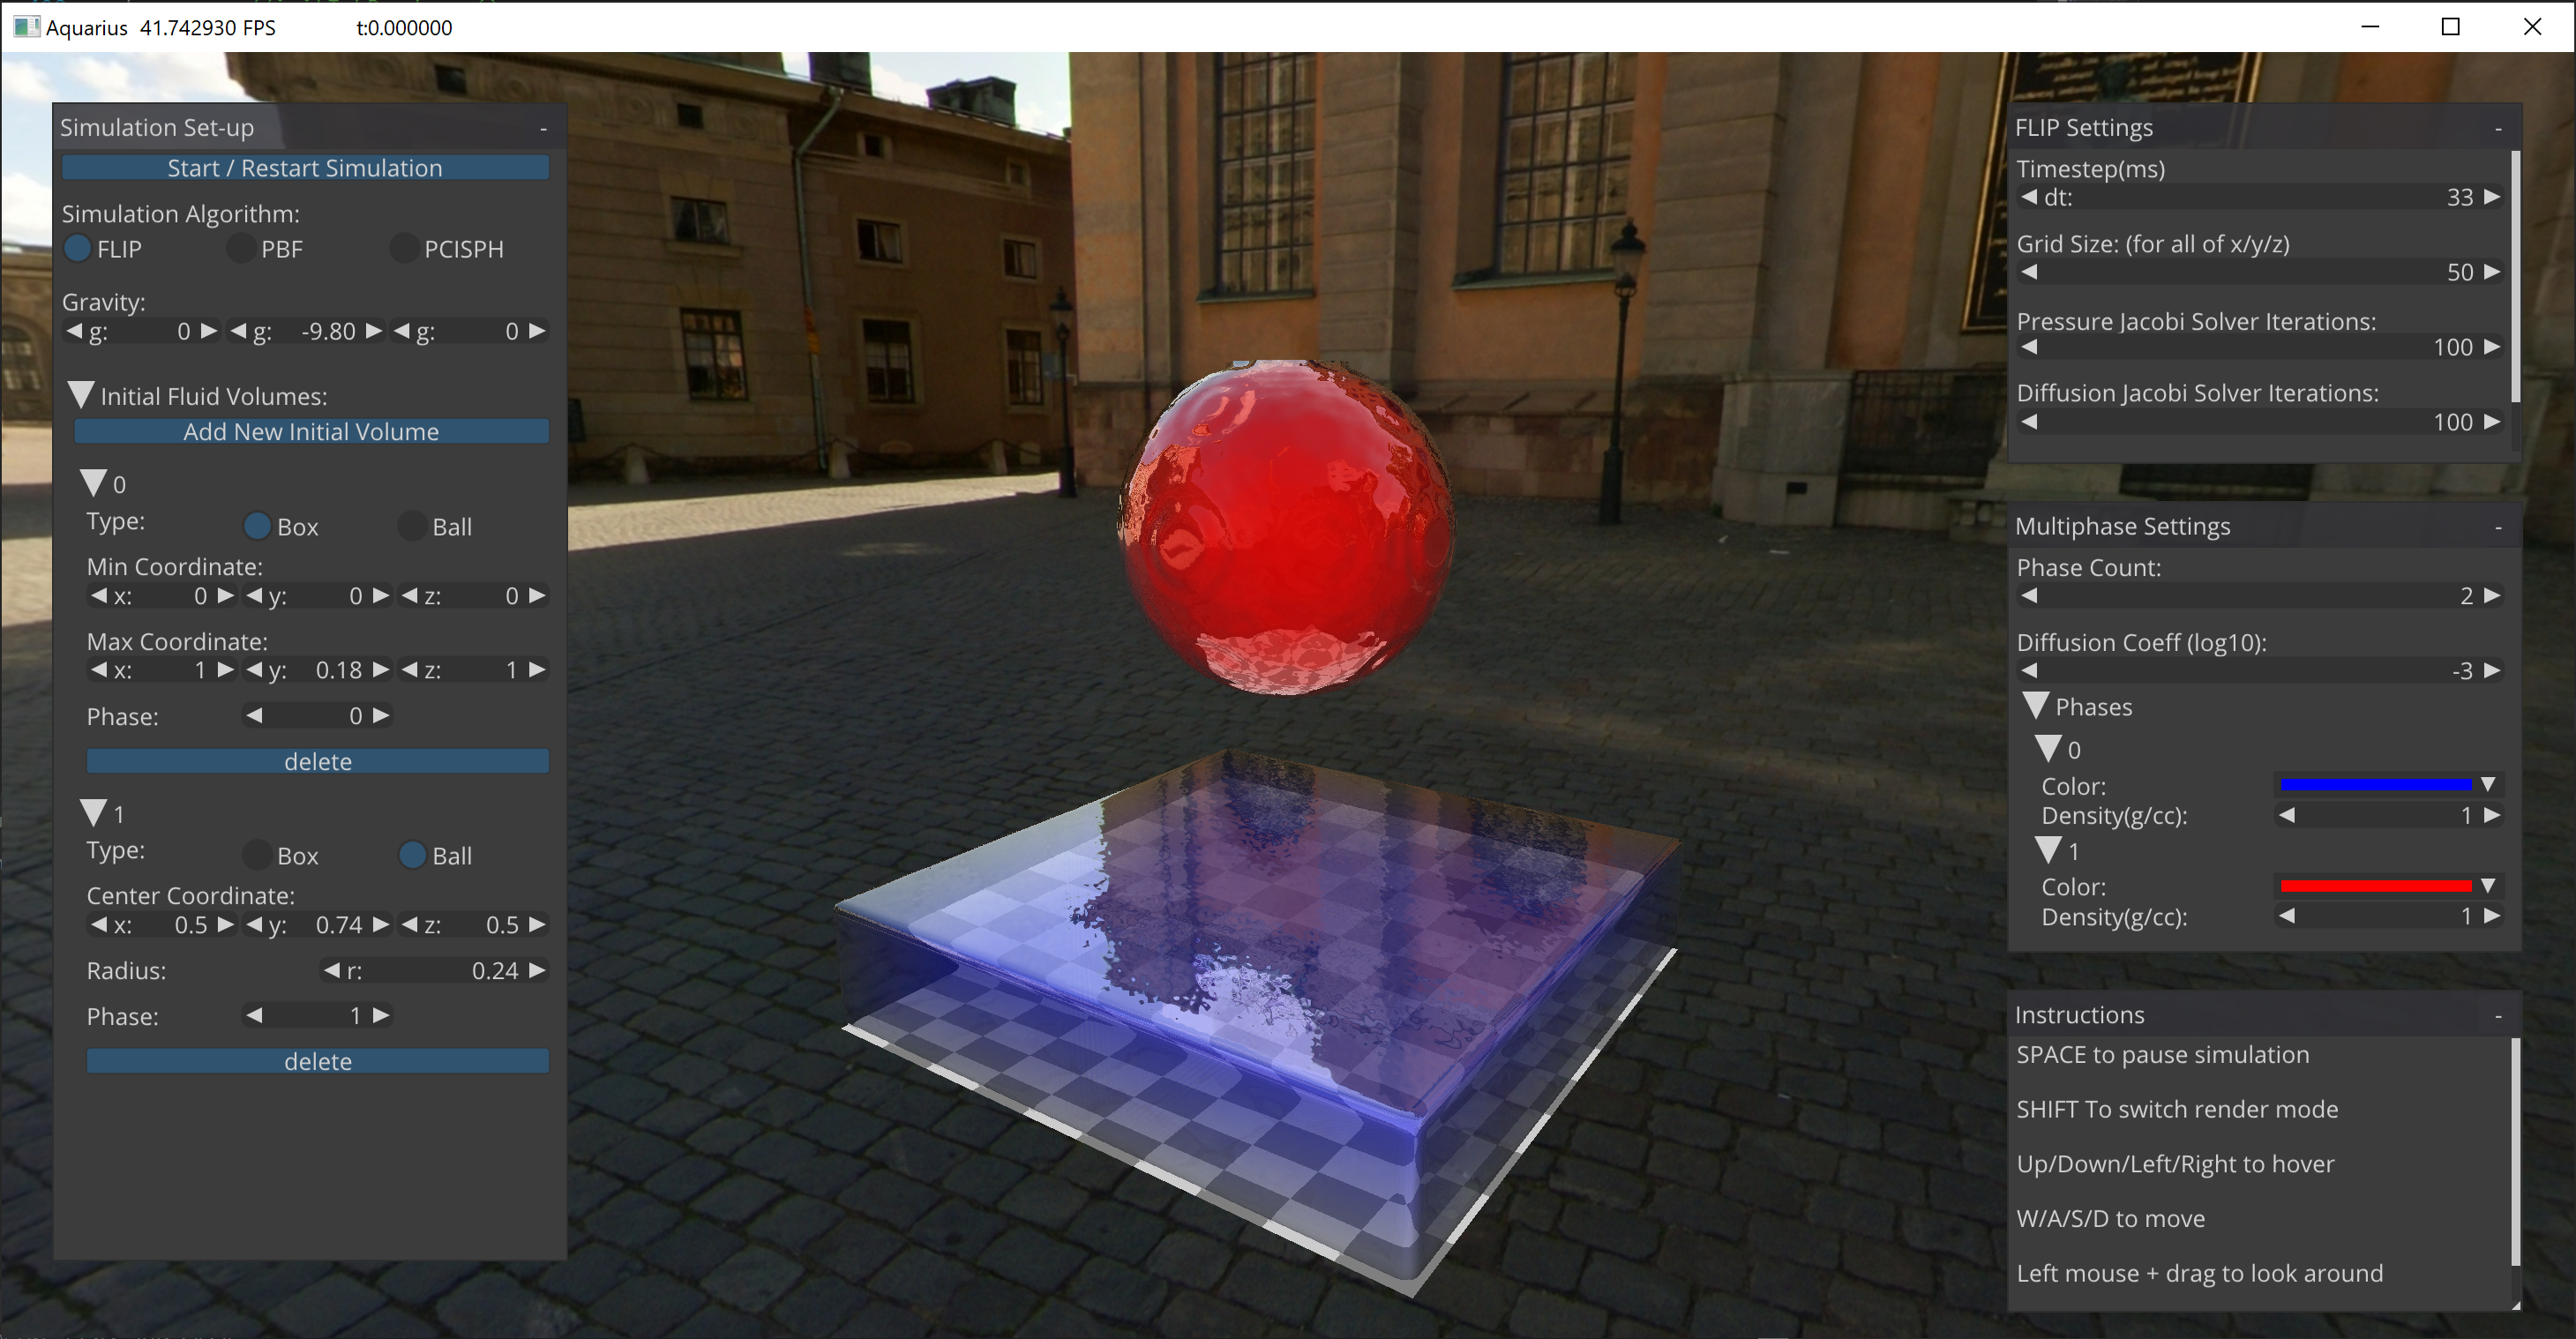
\includegraphics[width=15.2cm]{UI}
    \caption{The full user interface of the software}
    \label{figure UI demo}
\end{figure}
\chapter{Physics of Fluids}
\label{chapter physics}

The mechanics of fluids are governed by the partial differential equations (PDEs) known as the \textit{Incompressible Navier-Stokes Equations}, or in case of inviscid fluids, the \textit{Euler Equations}. This chapter explains the meaning and intuition behind these equations, which are key to designing and implementing numerical simulation algorithms.

\section{Vector Calculus}
The fluid equations are commonly written in the language of vector calculus. A brief introduction of the main concepts and operators involved is given in this chapter. 


\gapM

\textbf{Scaler Field}

\gapS

A \textit{scalar field} on $ \mathbb{R} ^3 $ is a mapping $\phi : \mathbb{R} ^3 \rightarrow \mathbb{R} $ from 3D cartesian coordinates to scalar values. Example scalar fields include fluid density, or pressure, where a scalar value can be sampled in each point of the 3D space.

\gapM

\textbf{Vector Field}

\gapS

A \textit{vector field} on $ \mathbb{R} ^3 $ is a mapping $\phi : \mathbb{R} ^3 \rightarrow \mathbb{R} ^3 $ from 3D cartesian coordinates to 3D vectors. A very commonly used vector field is the velocity field $\textbf{u}$, which describes the direction and speed of the fluid's movement at each point in the 3D space


\gapM

\textbf{The grad}

\gapS

Given a scalar field $\phi : \mathbb{R} ^3 \rightarrow \mathbb{R} $, the \textit{gradient} or \textit{grad} of the field is a vector field written as $\nabla \phi$, and it is defined by:
\begin{equation*}
    \nabla \phi = 
    \left(
    \begin{aligned}
        \frac{\partial \phi}{\partial x} \\
        \frac{\partial \phi}{\partial y} \\
        \frac{\partial \phi}{\partial z}
    \end{aligned} \right)
\end{equation*} 
The grad of a scalar quantity $\phi$ represents the rate of change of $\phi$ across each dimension. Moreover, $\nabla \phi$ computes the direction of movement which causes the greatest increase of $\phi$. 

\gapM

\textbf{The div}

\gapS

Given a vector field $\textbf{u} : \mathbb{R} ^3 \rightarrow \mathbb{R} ^3$, the \textit{divergence} or \textit{div} of the field is a scalar field written as $\nabla \cdot \textbf{u}$, and it is defined by:
$$
    \nabla \cdot \textbf{u} 
    = \nabla \cdot 
    \begin{pmatrix}
        \textbf{u}_x \\
        \textbf{u}_y \\
        \textbf{u}_z
    \end{pmatrix}
    =
    \frac{\partial \textbf{u}_x}{\partial x} +  
    \frac{\partial \textbf{u}_y}{\partial y} +
    \frac{\partial \textbf{u}_z}{\partial z}
$$
If $\textbf{u}$ is the velocity field, then the scalar field $\nabla \cdot \textbf{u}$ represents the speed at which the fluid is expanding or shrinking at each 3D location. Thus, a velocity field that satisfies $\nabla \cdot \textbf{u} = 0$ would keep the fluid in constant volume, which is how most fluids behave in the real world.


\gapM

\textbf{The curl}

\gapS

Given a vector field $\textbf{u} : \mathbb{R} ^3 \rightarrow \mathbb{R} ^3$, the \textit{curl} of the field is a scalar field written as $\nabla \cross \textbf{u}$, and it is defined by:
$$
    \nabla \cross \textbf{u} = 
    \nabla \cross \begin{pmatrix}
        \textbf{u}_x \\
        \textbf{u}_y \\
        \textbf{u}_z
    \end{pmatrix}
    =
    \left(
    \begin{aligned}
        \frac{\partial \textbf{u}_z}{\partial y} - 
            \frac{\partial \textbf{u}_y}{\partial z} \\
        \frac{\partial \textbf{u}_x}{\partial z} - 
            \frac{\partial \textbf{u}_z}{\partial x} \\
        \frac{\partial \textbf{u}_y}{\partial x} - 
            \frac{\partial \textbf{u}_x}{\partial y} \\
    \end{aligned} \right)
$$
Informally, the curl of the velocity field is a measure of the local rotation of the fluid. Though not directly used in the equations and algorithms presented in this project, it is at the heart of a different class of algorithms, called the vortex methods\cite{angelidis2005simulation}.


\gapM

\textbf{The Laplacian}

\gapS

The \textit{Laplacian} operator, written $\nabla \cdot \nabla$, is defined to be the divergence of the gradient. For scalar field $\phi$, it can be computed that:
$$
\nabla \cdot \nabla \phi = 
\frac{\partial ^2 \phi}{\partial x^2}+
\frac{\partial ^2 \phi}{\partial y^2}+
\frac{\partial ^2 \phi}{\partial z^2}
$$
The Laplacian describes the difference between the average value of $\phi$ in the neighborhood of a certain point and the value of $\phi$ at that point. As defined, this operator takes a scalar field and returns a scalar field. However, The Laplacian is also often extended to be applied to vector fields, where 
$$
\nabla \cdot \nabla \textbf{u} =
    \begin{pmatrix}
        \nabla \cdot \nabla \textbf{u}_x \\
        \nabla \cdot \nabla \textbf{u}_y \\
        \nabla \cdot \nabla \textbf{u}_z
    \end{pmatrix}
$$


\section{The Eulerian and Lagrangian Viewpoints}

For any physical quantity that represents some property of a fluid, the field of that quantity, either scalar or vector, could be constantly evolving as time passes. There are two different approaches to tracking this rate of change: the Eulerian viewpoint and the Lagrangian viewpoint.

The Eulerian viewpoint considers the time derivative of quantities at fixed locations in the 3D space. For a scalar field $\phi$ which varies through time, its \textit{Eulerian derivative} is simply $\dfrac{\partial \phi}{\partial t}$. To be more precise, the Eulerian derivative $\dfrac{\partial \phi}{\partial t}$, evaluated at point $\textbf{x}$, is the rate of change of $\phi$ of the fluid at the fixed position $\textbf{x}$, despite the fact that the fluid could be in motion. This has the immediate consequence that the concept of Eulerian derivative fails to capture the fact that physical quantities are carried around (i.e advected) by the fluid. 

The Lagrangian viewpoint, on the other hand, tracks the rates of changes of quantities as it moves along the velocity field $\textbf{u}$. In this approach, for a scalar field $\phi$, its derivative with respect to time is written as $\dfrac{D\phi}{Dt}$, and defined to be
$$
\frac{D\phi}{Dt} = \frac{\partial\phi}{\partial t} + \nabla \phi \cdot \textbf{u}
$$ 
This derivative, known as the \textit{Lagrangian derivative} or \textit{material derivative}, can be justified by treating the fluid as a collection of infinitesimal particles, each carrying some quantities and moving along the velocity field. At time $t$, for each particle $p$ with position $\textbf{x}$, the quantity of $\phi$ it carries is $\phi_p = \phi(t,\textbf{x}(p))$. The derivative with respect to $t$ of this term computes the rate of change of $\phi _p$:
$$
\begin{aligned}
    \frac{d}{dt} \phi_p
        &= \frac{d}{dt} \phi(t,\textbf{x}(t)) \\
        &= \frac{\partial \phi}{\partial t} + \nabla \phi \cdot \frac{d\textbf{x}}{dt} \\ 
        &= \frac{\partial \phi}{\partial t} + \nabla \phi \cdot \textbf{u} \\
        &=\frac{D\phi}{Dt}
\end{aligned}
$$
Which is precisely the Lagrangian derivative.

When formalizing the Euler and Navier-Stokes equations, the Lagrangian derivative $\dfrac{D}{Dt}$ will be automatically extended to be applied to vector fields, where each component of the vector field is differentiated separately. This allows the term $\dfrac{D\textbf{u}}{Dt}$ to be written, representing the acceleration of the infinitesimal fluid particles. 

As a flashforward to chapter \ref{chapter grid} and \ref{chapter particle}, the grid-based methods mainly employ the Eulerian viewpoint, storing quantities on a fixed grid, and using an explicit computational step called \textit{advection} to move around the quantities. In contrast, the particle-based methods always use the Lagrangian viewpoint, with quantities being recorded solely on particles.










\section{The Euler and Navier-Stokes Equations}
\label{Euler N-S Eqns}

Using the previously defined notations, the Euler equations, which governs the motion of an incompressible and inviscid fluid
%under gravity as the only external force
, can be written as

\begin{equation}
    \tag{Euler Equations}
    \left \{
    \begin{aligned}
         \frac{D\textbf{u}}{Dt}   &=   -\frac{\nabla p}{\rho} + \textbf{g} \\
         \nabla \cdot \textbf{u}   &=   0
    \end{aligned} \right.
    \label{eqn:Euler Equations}
\end{equation} 
where $\textbf{u}$ is the velocity field, $p$ is pressure, $\rho$ is the fluid's density, and $\textbf{g}$ the acceleration caused by an external force field (e.g gravity).

A generalized version of these equations is the famous incompressible Navier-Stokes equations, in which a term that describes viscosity is added:
\begin{equation}
    \tag{Navier-Stokes Equations}
    \left \{
    \begin{aligned}
         \frac{D\textbf{u}}{Dt}   &=   -\frac{\nabla p}{\rho} + \textbf{g} + \nu \nabla \cdot \nabla \textbf{u} \\
         \nabla \cdot \textbf{u}  &=   0
    \end{aligned} \right.
    \label{eqn:Navier-Stokes Equations}
\end{equation} 
where $\nu$ is the kinematic viscosity coefficient.


As described in the last section, the quantity $(\nabla \cdot \textbf{u})$ represents the rate at which the fluid is expanding or shrinking. Fluids in the real world usually remains in constant volume, unless in extreme conditions. This motivates the equation $\nabla \cdot \textbf{u} = 0$, included in both Euler and Navier-Stokes.


Besides the incompressibility condition, both Euler and Navier-Stokes include another equation known as the momentum equation (which is in fact a set of equations, because the quantities are vectors). The momentum equation essentially specifies Newton's 2nd law: $\textbf{a}$ = $\dfrac{\textbf{F}}{m}$ , i.e the acceleration is the force divided by the mass.

As previously explained, the quantity $\dfrac{D\textbf{u}}{Dt}$ represents the acceleration of the infinitesimal fluid particles. Thus, to explain the momentum equations, it remains to demonstrate that the right hand side correctly computes the force divided by the mass. Let the mass of the infinitesimal particle be $m$, and let the force be separated into the internal forces within the fluid $F_{in}$ and the external forces $F_{ext}$:
$$
\dfrac{D\textbf{u}}{Dt} = \frac{F_{in} + F_{ext}}{m}
$$
With $\textbf{g}$ representing the acceleration caused by an external force field (e.g gravity), this can be rewritten as
$$
\dfrac{D\textbf{u}}{Dt} = \frac{F_{in}}{m} + \textbf{g}
$$
The internal forces within a fluid is caused by an imbalance in pressure. Specifically, if one side of a infinitesimal particle has a greater pressure than the opposite side, then the particle will be pushed towards the low pressure region. This justifies why the pressure forces are in the direction of $-\nabla p$, which computes the direction of fastest decrease of pressure. From a dimensional analysis point of view, the unit of $p$ is $\dfrac{force}{length^2}$, thus the unit of $\nabla p$ is $\dfrac{force}{length^3}$. This indicates that to obtain the pressure force, it's necessary to multiply by the volume $V$ of the infinitesimal particle, which produces
$$
\dfrac{D\textbf{u}}{Dt} = -\frac{V \nabla p}{m} + \textbf{g}
$$
Using $\rho = \dfrac{m}{V}$, this becomes the Euler momentum equation:
$$
\dfrac{D\textbf{u}}{Dt} =  -\frac{\nabla p}{\rho} + \textbf{g}
$$



\chapter{Grid-Based Simulations}
\label{chapter grid}

This chapter introduces a grid-based multiphase fluid simulation scheme and its CUDA implementation in this project. This scheme has three key components: a \textbf{MAC} (Marker and Cell) grid for discretizing the Euler equations, a \textbf{FLIP} (Fluid Implicit Particle) algorithm for advection, and a Jacobi linear solver for solving the diffusion equation and the Poisson pressure equation (which ensures incompressibility).

\section{Operator Splitting}
\label{section splitting}
A common way for numerically solving differential equations is the \textit{operator splitting} approach. As a simple example, consider the simple differential equation:
$$
\frac{dx}{dt} = f(x)+g(x) ~~~~\mbox{With initial condition $x(0)=x_0$}
$$
To numerically solve this, decide on some small time step $\triangle t$, and let $x_{[n]}$ be the value of $x$ at the $n$th time step. The goal is to find $x_{[n]}$ for increasing larger $n$. To do this, start with $x_{[0]}=x_0$ and consider the two differential equations:
\begin{equation*}
    \begin{aligned}
        \frac{dx}{dt} = f(x)\\
        \frac{dx}{dt} = g(x)
    \end{aligned}
\end{equation*}
Suppose there exists some good solutions (either analytical or numerical) for these two equations, then these solutions can be used to find a good solution for the original equation. Specifically, suppose $F_{f_0}(t)$ is a solution of $\dfrac{dx}{dt} = f(x)$ with initial condition $x(0)=f_0$, and $G_{g_0}(t)$ is a solution of $\dfrac{dx}{dt} = g(x)$ with initial condition $x(0)=g_0$, then, the original equation can be solved as 
\begin{equation*}
    \begin{aligned}
        \widetilde{x} = F_{x_{[n]}}(\triangle t) \\
        x_{[n+1]} = G_{\widetilde{x}}(\triangle t) \\
    \end{aligned}
\end{equation*}
In essence, this approach splits the equation into a few more easily solved differential equations, and accumulates the solution of each over a small time step. 

This same splitting approach can be applied to the Euler equations. To do so, the Euler momentum equation is first written in a form where the material derivative is expanded using equation (\ref{Du/Dt}):
$$
\frac{\partial \u}{\partial t}   =  -\begin{pmatrix}
    \nabla \u_x  \cdot \u\\
     \nabla \u_y \cdot \u\\
     \nabla \u_z \cdot \u
  \end{pmatrix}
  + \textbf{g}
  -\frac{\nabla p}{\rho} 
$$
This then allows the equation, and therefore the simulation algorithm, to be split into three parts:
\begin{enumerate}
    \item
    $$
    \frac{\partial \u}{\partial t}   =  -\begin{pmatrix}
        \nabla \u_x  \cdot \u\\
         \nabla \u_y \cdot \u\\
         \nabla \u_z \cdot \u\end{pmatrix} 
    $$
    Again using equation (\ref{Du/Dt}), this can be rewritten back into the material derivative form:
    $$
    \dfrac{D\u}{Dt} = 0
    $$
    Intuitively, solving this equation means to move the fluid according to its velocity field, in a way such that the velocity of each infinitesimal fluid partial remains unchanged. This is the step known as \textit{advection}. 

    \item
    $$
    \frac{\partial \u}{\partial t}   = \textbf{g}
    $$
    Solving this equation is the process of exerting external forces (e.g gravity) on the fluid. The solid boundary conditions can also be enforced in this step.

    \item
    $$
    \frac{\partial \u}{\partial t}   = -\frac{\nabla p}{\rho} 
    $$
    Since this is the last step of the splitting, it is essential to make sure that the results of solving this equation satisfies the incompressibility condition $\nabla \cdot \u = 0$. This amounts to finding a pressure field $p$ such that, subtracting by $\triangle t \dfrac{\nabla p}{\rho}$ makes the velocity have zero divergence. This step enforces the incompressibility of the fluid.

\end{enumerate}



\section{Discretization}

The Euler equations involve two important quantities: the the pressure scalar field $p$, and the velocity vector field $\u$. For a numerical simulation, discretized versions of both fields need to maintained. A straightforward choice, which is used for the pressure field, is to maintain a 3d grid, where each cubic grid cell stores the pressure value sampled at the center of the cell. As an example, this figure shows the cell with location $(x,y,z)$, and 3 of its neighbors:


\begin{figure}[!h]
    \centering
    
    \tdplotsetmaincoords{-30}{0}
    \tdplotsetrotatedcoords{-0}{-20}{-0}

        \begin{tikzpicture}[tdplot_main_coords,tdplot_rotated_coords]

            

            
            \newcommand{\sizef}{4}
            \newcommand{\halff}{2}

            

            \draw[dashed] (0,0,0) -- (\sizef,0,0) ;
            \draw[dashed] (0,0,0) -- (0,\sizef,0);
            \draw[dashed] (0,0,0) -- (0,0,\sizef) ;

            \draw[dashed,->] (\sizef*2,0,0) -- (\sizef*2+1,0,0) node[right] {+x};
            \draw[dashed,->] (0,\sizef*2,0) -- (0,\sizef*2+1,0) node[above] {+y};
            \draw[dashed,->]  (0,0,\sizef*2) -- (0,0,\sizef*2+1) node[below] {+z};

            \foreach \x in {0,1}{
                \foreach \y in {0,1}{
                    \foreach \z in {0,1}{

                        

                        \pgfmathparse{
                            ifthenelse(equal(abs(\x)+abs(\y)+abs(\z),1),1,0) 
                        }

                        \ifthenelse{ 
                            \equal{\pgfmathresult}{1}
                            
                        }{

                            \foreach \a in {0,1}{
                                \foreach \b in {0,1}{
                                    \ifthenelse{\a  = 0 \AND \b = 0}{

                                        \draw [dashed]
                                        (
                                            \x * \sizef + \a * \sizef,
                                            \y * \sizef + \b * \sizef,
                                            \z * \sizef
                                        ) 

                                        -- 
                                        (
                                            \x * \sizef + \a * \sizef,
                                            \y * \sizef + \b * \sizef,
                                            \z * \sizef + \sizef
                                        ) ;
                                        
                                        \draw [dashed]
                                        (
                                            \x * \sizef + \a * \sizef,
                                            \y * \sizef,
                                            \z * \sizef + \b * \sizef,
                                        ) 

                                        -- 
                                        (
                                            \x * \sizef + \a * \sizef,
                                            \y * \sizef + \sizef,
                                            \z * \sizef + \b * \sizef,
                                        )  ;

                                        \draw [dashed]
                                        (
                                            \x * \sizef ,
                                            \y * \sizef + \a * \sizef,
                                            \z * \sizef + \b * \sizef,
                                        ) 

                                        -- 
                                        (
                                            \x * \sizef  + \sizef,
                                            \y * \sizef + \a * \sizef,
                                            \z * \sizef + \b * \sizef,
                                        )  ;
                                    
                                    }{
                                        \draw 
                                        (
                                            \x * \sizef + \a * \sizef,
                                            \y * \sizef + \b * \sizef,
                                            \z * \sizef
                                        ) 

                                        -- 
                                        (
                                            \x * \sizef + \a * \sizef,
                                            \y * \sizef + \b * \sizef,
                                            \z * \sizef + \sizef
                                        ) ;
                                        
                                        \draw 
                                        (
                                            \x * \sizef + \a * \sizef,
                                            \y * \sizef,
                                            \z * \sizef + \b * \sizef,
                                        ) 

                                        -- 
                                        (
                                            \x * \sizef + \a * \sizef,
                                            \y * \sizef + \sizef,
                                            \z * \sizef + \b * \sizef,
                                        )  ;

                                        \draw 
                                        (
                                            \x * \sizef ,
                                            \y * \sizef + \a * \sizef,
                                            \z * \sizef + \b * \sizef,
                                        ) 

                                        -- 
                                        (
                                            \x * \sizef  + \sizef,
                                            \y * \sizef + \a * \sizef,
                                            \z * \sizef + \b * \sizef,
                                        )  ;
                                    }

                                }
                            }

                        }{}

                        
                    }
                }
            }
            
            \node[draw,circle, fill, inner sep=1] at (\halff,\halff,\halff){};
            \node[below] at (\halff,\halff,\halff){\large{$p_{x,y,z}$}};

            \node[draw,circle, fill, inner sep=1] at (\halff+\sizef,\halff,\halff){};
            \node[below] at (\halff+\sizef,\halff,\halff){\large{$p_{x+1,y,z}$}};

            \node[draw,circle, fill, inner sep=1] at (\halff,\halff+\sizef,\halff){};
            \node[below] at (\halff,\halff+\sizef,\halff){\large{$p_{x,y+1,z}$}};

            \node[draw,circle, fill, inner sep=1] at (\halff,\halff,\halff+\sizef){};
            \node[below] at (\halff,\halff,\halff+\sizef){\large{$p_{x,y,z+1}$}};


        
         \end{tikzpicture}
    
    \label{pressure cell}
\end{figure}
Other than being simple to understand and implement, this discretization scheme also has the advantage that the finite difference approximation of the Laplacian of the pressure field, sampled at the center of the cells, can be easily computed:

\begin{equation}
    \begin{aligned}
        \nabla \cdot \nabla p 
        &= 
        \frac{\partial ^2 p}{\partial x^2}+
        \frac{\partial ^2 p}{\partial y^2}+
        \frac{\partial ^2 p}{\partial z^2} \\
        &\approx 
        \frac{p_{x+1,y,z}+p_{x-1,y,z}-2p_{x,y,z}}{(\triangle x)^2}+ \\
        &~~~~\frac{p_{x,y+1,z}+p_{x,y-1,z}-2p_{x,y,z}}{(\triangle x)^2}+ \\
        &~~~~\frac{p_{x,y,z+1}+p_{x,y,z-1}-2p_{x,y,z}}{(\triangle x)^2}\\
        &= \frac{p_{x+1,y,z}+p_{x-1,y,z}+p_{x,y+1,z}+p_{x,y-1,z}+p_{x,y,z+1}+p_{x,y,z-1}-6p_{x,y,z}}{(\triangle x)^2}
    \end{aligned}
    \label{eqn discrete laplacian pressure}
\end{equation}
where $\triangle x$ is the edge length of the cubic cell. 


For the velocity field $\u$, a slightly more sophisticated method known as the \textbf{MAC}(Marker and Cell) grid is used. Instead of storing the value of $\u = (\u_x,\u_y,\u_z)$ sampled at the cell center, an MAC grid stores different components of $\u$ sampled at different locations. Specifically, the grid cell at position $(x,y,z)$ stores the value of $\u_x$ sampled at the center of its left face, the value of $\u_y$ sampled at its lower face, and the value of $\u_z$ sampled at its back face, as illustrated in this figure:

\begin{figure}[!h]
    \centering
        \begin{tikzpicture} 

            \newcommand{\sizef}{4}
            \newcommand{\halff}{2}

            \draw[dashed,->] (0,0,0) -- (\sizef + 1,0,0) node[right] {+x};
            \draw[dashed,->] (0,0,0) -- (0,\sizef + 1,0) node[above] {+y};
            \draw[dashed,->] (0,0,0) -- (0,0,\sizef + 1) node[below] {+z};


            \foreach \a in {0,1}{
                \foreach \b in {0,1}{
                    \ifthenelse{  \a  = 0 \AND \b = 0  }
                    {
                        \draw[dashed] (\a * \sizef,\b * \sizef,0) 
                        -- (\a * \sizef,\b * \sizef,\sizef);

                        \draw[dashed] (\a * \sizef,0,\b * \sizef) 
                            -- (\a * \sizef,\sizef,\b * \sizef);

                        \draw[dashed] (0,\a * \sizef,\b * \sizef) 
                            -- (\sizef,\a * \sizef,\b * \sizef);
                    }
                    {

                        \draw (\a * \sizef,\b * \sizef,0) 
                        -- (\a * \sizef,\b * \sizef,\sizef);

                        \draw (\a * \sizef,0,\b * \sizef) 
                            -- (\a * \sizef,\sizef,\b * \sizef);

                        \draw (0,\a * \sizef,\b * \sizef) 
                            -- (\sizef,\a * \sizef,\b * \sizef);
                    }

                }
            }

            

            \node[draw,circle, fill, inner sep=1] at (\halff,\halff,0){};
            \node[below] at (\halff,\halff,0){\large{$\u_{x,y,z-\frac{1}{2}}$}};

           

            \node[draw,circle, fill, inner sep=1] at (\halff,0,\halff){};
            \node[below] at (\halff,0,\halff){\large{$\u_{x,y-\frac{1}{2},z}$}};

            
            \node[draw,circle, fill, inner sep=1] at (0,\halff,\halff){};
            \node[below] at (0,\halff,\halff){\large{$\u_{x-\frac{1}{2},y,z}$}};
           
        

            % \node[draw,circle, fill, inner sep=1] at (\halff,\halff,\sizef){};
            % \node[right] at (\halff,\halff,\sizef){\large{$\u_{x,y,z+\frac{1}{2}}$}};

            % \node[draw,circle, fill, inner sep=1] at (\halff,\sizef,\halff){};
            % \node[above] at (\halff,\sizef,\halff){\large{$\u_{x,y+\frac{1}{2},z}$}};

            % \node[draw,circle, fill, inner sep=1] at (\sizef,\halff,\halff){};
            % \node[right] at (\sizef,\halff,\halff){\large{$\u_{x+\frac{1}{2},y,z}$}};

        
         \end{tikzpicture}
    
    \caption{a 3D MAC grid cell and the velocity data it stores}
    \label{mac cell 1}
\end{figure}


The quantities $\u_{x,y,z-\frac{1}{2}}$, $\u_{x,y-\frac{1}{2},z}$, $\u_{x-\frac{1}{2},y,z}$ are all scalars, representing the velocity pointing at the $x$, $y$, and $z$ direction, respectively. Furthermore, notice that the values of $\u_{x+\frac{1}{2},y,z}$, $\u_{x,y+\frac{1}{2},z}$, and $\u_{x,y,z+\frac{1}{2}}$, which are respectively sampled at the centers of the right, upper, and front faces, will also be available. This is because $\u_{x+\frac{1}{2},y,z} = \u_{x+1-\frac{1}{2},y,z}$, that is, the value of $\u_x$ sampled at the right face of the cell is exactly the value of $\u_x$ sampled at the left face of the neighboring cell on the right. The same can be applied for the upper and front faces. As a result, there are 6 velocity values associated with each grid cell:

\begin{figure}[!h]
    \centering
        \begin{tikzpicture} 

            \newcommand{\sizef}{4}
            \newcommand{\halff}{2}

            \draw[dashed,->] (0,0,0) -- (\sizef + 1,0,0) node[right] {+x};
            \draw[dashed,->] (0,0,0) -- (0,\sizef + 1,0) node[above] {+y};
            \draw[dashed,->] (0,0,0) -- (0,0,\sizef + 1) node[below] {+z};


            \foreach \a in {0,1}{
                \foreach \b in {0,1}{
                    \ifthenelse{  \a  = 0 \AND \b = 0  }
                    {
                        \draw[dashed] (\a * \sizef,\b * \sizef,0) 
                        -- (\a * \sizef,\b * \sizef,\sizef);

                        \draw[dashed] (\a * \sizef,0,\b * \sizef) 
                            -- (\a * \sizef,\sizef,\b * \sizef);

                        \draw[dashed] (0,\a * \sizef,\b * \sizef) 
                            -- (\sizef,\a * \sizef,\b * \sizef);
                    }
                    {

                        \draw (\a * \sizef,\b * \sizef,0) 
                        -- (\a * \sizef,\b * \sizef,\sizef);

                        \draw (\a * \sizef,0,\b * \sizef) 
                            -- (\a * \sizef,\sizef,\b * \sizef);

                        \draw (0,\a * \sizef,\b * \sizef) 
                            -- (\sizef,\a * \sizef,\b * \sizef);
                    }

                }
            }

            \node[draw,circle, fill, inner sep=1] at (\halff,\halff,0){};
            \node[below] at (\halff,\halff,0){\large{$\u_{x,y,z-\frac{1}{2}}$}};

           

            \node[draw,circle, fill, inner sep=1] at (\halff,0,\halff){};
            \node[below] at (\halff,0,\halff){\large{$\u_{x,y-\frac{1}{2},z}$}};

            
            \node[draw,circle, fill, inner sep=1] at (0,\halff,\halff){};
            \node[below] at (0,\halff,\halff){\large{$\u_{x-\frac{1}{2},y,z}$}};

            
            \node[draw,circle, fill, inner sep=1] at (\halff,\halff,\sizef){};
            \node[right] at (\halff,\halff,\sizef){\large{$\u_{x,y,z+\frac{1}{2}}$}};

            \node[draw,circle, fill, inner sep=1] at (\halff,\sizef,\halff){};
            \node[above] at (\halff,\sizef,\halff){\large{$\u_{x,y+\frac{1}{2},z}$}};

            \node[draw,circle, fill, inner sep=1] at (\sizef,\halff,\halff){};
            \node[right] at (\sizef,\halff,\halff){\large{$\u_{x+\frac{1}{2},y,z}$}};

        
         \end{tikzpicture}
    
    \label{mac cell 2}
\end{figure}

Using these quantities, an approximation of the divergence of the velocity, $\nabla \cdot \u$, sampled at cell centers, can be easily computed:
\begin{equation}
    \begin{aligned}
        \nabla \cdot \u 
        &=
        \frac{\partial \u_x}{\partial x} +  
        \frac{\partial \u_y}{\partial y} +
        \frac{\partial \u_z}{\partial z} \\
        &\approx 
        \frac{\triangle \u_x}{\triangle x} +  
        \frac{\triangle \u_y}{\triangle y} +
        \frac{\triangle \u_z}{\triangle z}\\
        &= 
        \frac{\u_{x+\frac{1}{2},y,z} - \u_{x-\frac{1}{2},y,z}}{\triangle x} +  
        \frac{\u_{x,y+\frac{1}{2},z} - \u_{x,y-\frac{1}{2},z}}{\triangle x} +
        \frac{\u_{x,y,z+\frac{1}{2}} - \u_{x,y,z-\frac{1}{2}}}{\triangle x}
    \end{aligned}
    \label{eqn discrete div u}
\end{equation}

During the incompressibility step of the simulation, the velocity field will be updated according the gradient of the pressure field. Thus, it's also important to compute the approximation of $\nabla p$ at the velocity field sample points, i.e the centers of faces of the cells. This is made easy by the fact that, the pressure field is sampled at the centers of the cells:
\begin{equation}
    \label{eqn discrete grad p}
    \begin{aligned}
        (\nabla p)_{x-\frac{1}{2},y,z} = \frac{p_{x,y,z}-p_{x-1,y,z}}{\triangle x}
    \end{aligned}
\end{equation}
The numerical approximations to $\nabla \cdot \nabla p$, $\nabla \cdot \u$, and $\nabla p$ will all be used during the incompressibility step, as will be explained in section \ref{section enforce incompressibility}.

\section{Advection}

As previously explained, the first step in each time step of the simulation is to solve the advection equation $\dfrac{D\u}{Dt} = 0$. Intuitively, this equation demands that the velocity of each infinitesimal particle in the fluid remains unchanged (but the velocity field itself will change because the positions of the particles will change).

A once widely used advection algorithm is called \textbf{PIC}(Particle in Cell), which is closely based on the intuition behind the material derivative. Instead of infinitely many infinitely small particles, the fluid is approximately represented using a finite but large cloud of particles, each storing its own velocity. Using the velocity field $\u_{[n]}$ in $n$th time step, the PIC advection at the $n+1$ th time step work in these following steps: 

\begin{enumerate}
    \item For each particle $p$ with position $\textbf{x}_p$, sample and interpolate the MAC grid to obtain the value of $\u_{[n]}$ at $\textbf{x}_p$. Assign this as the particle's velocity,  $\u_p$.
    
    \item Move the particle in the velocity field $\u_{[n]}$. This can be as simple as computing $\textbf{x}_p^{new} = \textbf{x}_p + \triangle t \u_{[n]}(\textbf{x}_p)$. For higher accuracy, this project performs this using a 3rd-order Runge-Kutta integration:
    \begin{equation*}
        \begin{aligned}
            \u_{temp1} &= \u_{[n]}(\textbf{x}_p) \\
            \u_{temp2} &= \u_{[n]}(\textbf{x}_p + \frac{1}{2}\triangle t \u_{temp1}) \\
            \u_{temp3} &= \u_{[n]}(\textbf{x}_p + \frac{3}{4}\triangle t \u_{temp2})\\
            \textbf{x}_p^{new} &=  \textbf{x}_p + \triangle t(
                \frac{2}{9}\u_{temp1} + \frac{3}{9}\u_{temp2} + \frac{4}{9}\u_{temp3}
                )
        \end{aligned}
    \end{equation*}
    For particles near the boundaries of the fluid, some of the $\u_{temp}$ values might be sampled outside the fluid region, which is slightly problematic because the velocity isn't defined outside the fluids. This is fixed by a simple \textit{extrapolation} step, which extends the velocity to a few grid cells outside its original region.
    
    
    \item For each MAC grid cell, and for each of its 3 sample points where a component of $\u$ is stored, find all particles within a certain small radius (usually $\triangle x$), and interpolate their value of $\u_p$. Save these values as a temporary velocity field, $\u_{[n+1]}^{advected}$.
\end{enumerate}
In short, the PIC algorithm first transfers the velocity field from the MAC grid to the particles, then move the particles, and then transfers the velocity from the particles back to the MAC grid.



The PIC algorithm is largely superseded by another algorithm known as \textbf{FLIP}(Fluid Implicit Particle), which is implemented in this project. FLIP is very similar to PIC, with only a slightly different 1st step:
\begin{enumerate}
    \item [$1'.$]
    For each particle $p$ with position $\textbf{x}_p$, sample and interpolate the MAC grid to obtain the value of $\u_{[n]} - \u_{[n-1]}$ at $\textbf{x}_p$. Add this to the particle's velocity,  $\u_p$.
\end{enumerate}
That is, instead of interpolating the value of $\u$ on to the particles, FLIP interpolates the change of $\u$ in the last time step, and add that to the particles' velocities. Zhu and Bridson \cite{zhu2005animating} showed that this method reduces the undesirable effect called \textit{numerical dissipation}, where visually interesting details in the fluid are smoothed away due to excessive interpolation.



\section{External Forces}

After obtaining the temporary velocity field $\u_{[n+1]}^{advected}$, the next step is to apply external forces. Two types of external forces will be considered: the forces arising from an external force field such as gravity, and the forces exerted by a solid boundary.

Let $\textbf{g}$ denote the acceleration caused by the external force field, (for gravity, $\textbf{g}\approx[0,-0.98,0]^T$), applying the forces is then achieved by adding $\triangle t \textbf{g}$. In a MAC grid, this is done by updating the components of $\u$ sampled at different faces using the different components of $\triangle t \textbf{g}$. 


To apply the solid boundary condition $\u \cdot \textbf{n} = 0$, as mentioned in section \ref{section boundary conditions}, components of $\u$ sampled at faces that represent solid-fluid boundaries need to be set to 0. For example, if the solid region is considered to be exactly the region of space outside the MAC grid, then the leftmost faces of the leftmost cells (and rightmost faces of rightmost cells...etc) will be considered as a solid-fluid boundary. For all such boundary faces, the velocity component there will be set to 0. 

Starting from an incompressible velocity field $\u_{[n]}$, performing advection to obtain $\u_{[n+1]}^{advected}$, and then applying external forces, the resulting velocity will likely not be incompressible anymore. Let this field be called $\u_{[n+1]}^{compressible}$, and the next step will be to apply pressure within the fluid, so that the incompressibility is restored.


\section{Enforcing Incompressibility}
\label{section enforce incompressibility}
To enforce the incompressibility condition $\nabla \cdot \u_{[n+1]} = 0$, the algorithm needs to find a pressure field $p$ such that,
\begin{equation*}
    \begin{aligned}
        \nabla \cdot \u_{[n+1]} = \nabla \cdot
        ( \u_{[n+1]}^{compressible} - \triangle t \frac{\nabla p}{\rho} ) = 0
    \end{aligned}
\end{equation*}
Rearranging the equation on the right gives
$$
-\frac{\triangle t}{\rho} \nabla \cdot \nabla p = -\nabla \cdot \u_{[n+1]}^{compressible}
$$
Using the discretization formulas \ref{eqn discrete laplacian pressure} and \ref{eqn discrete div u}, the discrete version of this equation can be written: 
\begin{equation*}
    \begin{aligned}
        \frac{\triangle t}{\rho \triangle x}(6p_{x,y,z}-p_{x+1,y,z}-p_{x-1,y,z}-p_{x,y+1,z}-p_{x,y-1,z}-p_{x,y,z+1}-p_{x,y,z-1}) \\
        = 
        -( \u_{x+\frac{1}{2},y,z} - \u_{x-\frac{1}{2},y,z}  +  
         \u_{x,y+\frac{1}{2},z} - \u_{x,y-\frac{1}{2},z} +
         \u_{x,y,z+\frac{1}{2}} - \u_{x,y,z-\frac{1}{2}})
    \end{aligned}
\end{equation*}
One such equation exists for every cell that contains fluid (i.e contains FLIP particles), and together, they form a system of linear equations, called the \textit{Poisson pressure equation}. The unknowns, $p_{i,j,k}$, correspond to the pressure at the centers of cells.

Since each equation involves not only the pressure of the fluid cell itself, but also the pressure of its 6 adjacent cells, extra care needs to be taken for cells that are at the boundaries of the fluid. Specifically, if a variable $p_{i,j,k}$ in the equations corresponds to the pressure within a air cell, it should automatically be assigned 0, which satisfies the free surface boundary conditions. If the variable $p_{i,j,k}$ corresponds to the pressure within solid, then it suffices to replace it with the pressure of the fluid cell next to the boundary, because the velocities at solid-fluid boundaries were already fixed in the external forces step.

With the boundary conditions satisfied, the equation become a system of $N$ linear equations with $N$ variables, where $N$ is the total amount of fluid cells. Solving this system hence results in a discrete representation of the pressure field $p$ that satisfies 
$$
\nabla \cdot
 ( \u_{[n+1]}^{compressible} - \triangle t \frac{\nabla p}{\rho} ) = 0
$$
Then, to retrieve the incompressible velocity field, it only remains to compute
$$ \u_{[n+1]} = \u_{[n+1]}^{compressible} - \triangle t \frac{\nabla p}{\rho}$$
using discretization formula \ref{eqn discrete div u}. This completes the simulation of one time step.

\gapM

To summarize, using a grid and FLIP advection, the simulation of each time step follows the following procedure:

\begin{algorithm}[H]
    \label{algo singlephase flip}

    \SetAlgoLined
    \tcp{At time step [n+1]}
    \ForEach{particle $p$}{
        $\u_p := \u_p + \u_{[n]}(\textbf{x}_p) - \u_{[n-1]}(\textbf{x}_p)$ \;
        Move $p$ inside the velocity field using Runge-Kutta\;
    }
    \ForEach{grid cell at location $(x,y,z)$}{
        Find all particles within a radius of $\triangle x$\;
        Compute $\u_{[n+1]}^{advected}$, as an interpolation of the $\u_p$ of nearby particles\;
    }
    Apply external forces, $\u_{[n+1]}^{compressible} =  FixSolidBoundary(u_{[n+1]}^{advected} + \triangle t \textbf{g})$\;
    Construct and solve the Poisson pressure equation, obtain pressure $p$\;
    Compute $\u_{[n+1]} = \u_{[n+1]}^{compressible} - \triangle t \dfrac{\nabla p}{\rho}$

    \caption{Single phase fluid FLIP simulation step}
\end{algorithm}


\section{Simulating Diffusion}
While algorithm \ref{algo singlephase flip} is only for single phase fluid simulation, it is possible to extend it to support multiple fluid phases. As explained in section \ref{section multiple fluids}, the changes in the concentration $\alpha^i$ of a fluid phase $i$ is governed by the Advection-Diffusion equation:
$$
\frac{D \alpha^i}{D t} = C\nabla \cdot \nabla \alpha^i
$$
To incorporate this equation to the simulation algorithm, the first step is again to apply splitting. The equation is split into two parts:
\begin{equation*}
    \begin{aligned}
        \frac{D \alpha^i}{D t} &= 0\\
        \frac{\partial \alpha^i}{\partial t} &= C\nabla \cdot \nabla \alpha^i
    \end{aligned}
\end{equation*}
Just like the Euler momentum equation, this first equation that splitting produces is an advection equation. Thus, the same FLIP advection that was applied for the velocity field can be used to advect the concentration quantities: first transfer the quantities from the grid to the particles by interpolating and adding $\alpha^{i}_{[n]} - \alpha^{i}_{[n-1]}$, then move the particles in the velocity field, then transfer the $\alpha^i$ back to the grid. 

The second equation is the "diffusion" part of the advection-diffusion equation, and is sometimes referred as the diffusion equation by itself. It was shown that using forward Euler scheme for this equation is unstable for large time steps\cite{kang2010hybrid}, so a discretized implicit equation is used:
\begin{equation*}
    \begin{aligned}
        - \lambda\alpha^i_{[n+1]~x-1,y,z}
        - \lambda\alpha^i_{[n+1]~x+1,y,z}\\
        - \lambda\alpha^i_{[n+1]~x,y-1,z}
        - \lambda\alpha^i_{[n+1]~x,y+1,z}\\
        - \lambda\alpha^i_{[n+1]~x,y,z-1}
        - \lambda\alpha^i_{[n+1]~x,y,z+1}\\
        +(1+6\lambda)\alpha^i_{[n+1] x,y,z} 
    \end{aligned}
    ~~=~~ \alpha^{i,advected}_{[n] x,y,z} 
\end{equation*}
where $\lambda = \dfrac{C\triangle t}{(\triangle x)^2}$. With the value of $\alpha^i_{n+1}$ at each fluid cell as unknown, this is again a linear equation. Solving the equation produces the new concentration field, $\alpha^i_{[n+1]}$.

Incorporating the FLIP concentration advection and solving the diffusion equation into the previous algorithm gives an algorithm for multiphase simulation:

\begin{algorithm}[H]
    \label{algo multiphase flip}

    \SetAlgoLined
    \tcp{At time step [n+1]}
    \ForEach{particle $p$}{
        $\u_p := \u_p + \u_{[n]}(\textbf{x}_p) - \u_{[n-1]}(\textbf{x}_p)$ \;
        $\alpha_p^i := \alpha_p^i + \alpha^i_{[n]}(\textbf{x}_p) - \alpha^i_{[n-1]}(\textbf{x}_p)$, for all fluid phases $i$ \;
        Move $p$ inside the velocity field using Runge-Kutta\;
    }
    \ForEach{grid cell at location $(x,y,z)$}{
        Find all particles within a radius of $\triangle x$\;
        Compute $\u_{[n+1]}^{advected}$, as an interpolation of the $\u_p$ of nearby particles\;
        Compute $\alpha_{[n+1]}^{advected}$, as an interpolation of the $\alpha _p$ of nearby particles\;
    }
    Apply external forces, $\u_{[n+1]}^{compressible} =  FixSolidBoundary(u_{[n+1]}^{advected} + \triangle t \textbf{g})$\;
    Construct and solve the Poisson pressure equation, obtain pressure $p$\;
    Compute $\u_{[n+1]} = \u_{[n+1]}^{compressible} - \triangle t \dfrac{\nabla p}{\rho}$\;
    Construct and solve the discretized diffusion equation to obtain $\alpha^i_{n+1}$ for all fluid phases $i$.

    \caption{Multiphase phase fluid FLIP simulation step}
\end{algorithm}



\section{Implementation}

The pseudocode presentation of algorithm \ref{algo multiphase flip} takes a sequential form, and the challenge remains to parallelize this algorithm on GPU. 

For certain parts of the algorithm, parallelization is straightforward. This includes line 2-4, line 8-9, which are all operations performed within a loop body. In different loop iterations, the data being operated on are completely different, and does not depend on previous iterations, which means it is safe to use parallel threads instead of loops to perform these operations. Similarly, the velocity field updates in line 11 and 13 are also easy to parallelize, with each thread operating on one grid cell of the discretized velocity field. 

The rest of the algorithm, line 7, 12 and 14, requires much more attention. Line 7 performs a task called \textit{spatial indexing}: associating each grid cell with all the particles that are within radius $\triangle x$ at each time step. A naive implementation would require a linear search on all particles, and this has to be performed for all grid cells, which is intolerable because the simulation could involve up to around 1,000,000 particles and 100,000 grid cells. In line 12 and 14, a linear equation needs to be solved, where there's an unknown for each fluid cell. As a result, the total amount of unknowns is in the order of 100,000. A naive linear solver have a $O(N^3)$ complexity, which is also too costly. In order to achieve real-time simulation and rendering, each of these operations, indexing 1,000,000 million particles and solving linear equations with 100,000 unknowns, needs to be performed at least around 20 times per second. This section will focus on how this is made possible in this project.

\subsection{Spatial Indexing}
\label{subsection spatial indexing}
With $\triangle x$ being the edge length of each cubic grid cell, finding all particles within a radius $\triangle x$ of each cell can be reduced to finding the particles that are \textit{inside} each cell. Then, for a certain cell, it suffices to check all the 27 cells in the neighborhood, because all particles within a radius $\triangle x$ must be contained inside these 27 cells. 


To create an index from each cell to the particles inside the cell, this project uses the parallel algorithm proposed by Green \cite{harlow1965numerical}. The algorithm proceeds in the following steps:

\begin{figure}[p]
    \begin{minipage}[t]{.65\linewidth}
        \vspace{0pt}
        \centering
        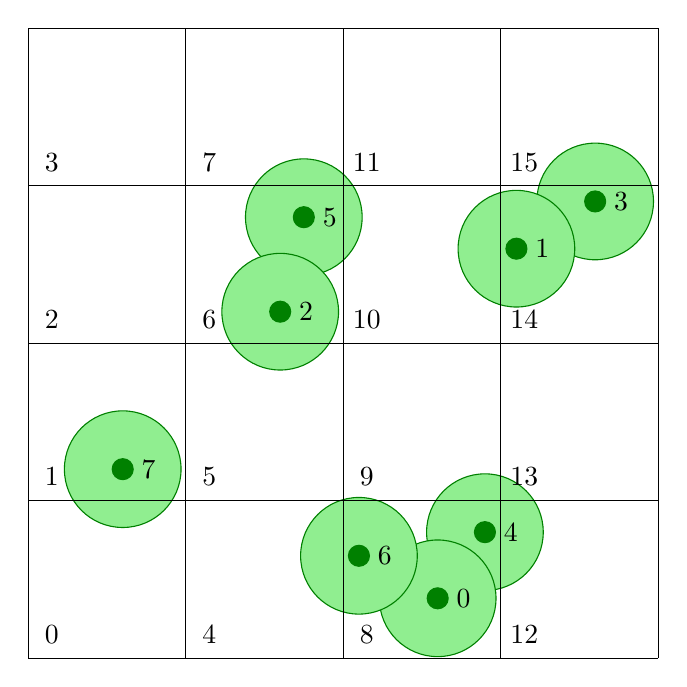
\begin{tikzpicture} 
            \pgfmathsetmacro\dx{2};
            \pgfmathsetmacro\radius{\dx / 2.7};
            \pgfmathsetmacro\centerRadius{\dx / 15};

            \pgfmathsetmacro\x{0.6*\dx};
            \pgfmathsetmacro\y{1.2*\dx};
            \filldraw[draw=Green,fill=LightGreen] (\x,\y) circle (\radius);
            \filldraw[draw=Green,fill=Green] (\x,\y) circle (\centerRadius) node[right]{~7};

            \pgfmathsetmacro\x{1.75*\dx};
            \pgfmathsetmacro\y{2.8*\dx};
            \filldraw[draw=Green,fill=LightGreen] (\x,\y) circle (\radius);
            \filldraw[draw=Green,fill=Green] (\x,\y) circle (\centerRadius)node[right]{~5};

            \pgfmathsetmacro\x{1.6*\dx};
            \pgfmathsetmacro\y{2.2*\dx};
            \filldraw[draw=Green,fill=LightGreen] (\x,\y) circle (\radius);
            \filldraw[draw=Green,fill=Green] (\x,\y) circle (\centerRadius)node[right]{~2};

            \pgfmathsetmacro\x{2.9*\dx};
            \pgfmathsetmacro\y{0.8*\dx};
            \filldraw[draw=Green,fill=LightGreen] (\x,\y) circle (\radius);
            \filldraw[draw=Green,fill=Green] (\x,\y) circle (\centerRadius)node[right]{~4};

            \pgfmathsetmacro\x{2.6*\dx};
            \pgfmathsetmacro\y{0.38*\dx};
            \filldraw[draw=Green,fill=LightGreen] (\x,\y) circle (\radius);
            \filldraw[draw=Green,fill=Green] (\x,\y) circle (\centerRadius)node[right]{~0};

            \pgfmathsetmacro\x{2.1*\dx};
            \pgfmathsetmacro\y{0.65*\dx};
            \filldraw[draw=Green,fill=LightGreen] (\x,\y) circle (\radius);
            \filldraw[draw=Green,fill=Green] (\x,\y) circle (\centerRadius)node[right]{~6};

            \pgfmathsetmacro\x{3.6*\dx};
            \pgfmathsetmacro\y{2.9*\dx};
            \filldraw[draw=Green,fill=LightGreen] (\x,\y) circle (\radius);
            \filldraw[draw=Green,fill=Green] (\x,\y) circle (\centerRadius)node[right]{~3};

            \pgfmathsetmacro\x{3.1*\dx};
            \pgfmathsetmacro\y{2.6*\dx};
            \filldraw[draw=Green,fill=LightGreen] (\x,\y) circle (\radius);
            \filldraw[draw=Green,fill=Green] (\x,\y) circle (\centerRadius)node[right]{~1};

            

            \foreach \x in {0,1,2,3}{
                \foreach \y in {0,1,2,3}{  
                    \draw (\x*\dx,\y*\dx) -- (\x*\dx+\dx,\y*\dx);
                    \draw (\x*\dx,\y*\dx) -- (\x*\dx,\y*\dx+\dx);
                    \draw (\x*\dx+\dx,\y*\dx) -- (\x*\dx+\dx,\y*\dx+\dx);
                    \draw (\x*\dx,\y*\dx+\dx) -- (\x*\dx+\dx,\y*\dx+\dx);
                    \pgfmathtruncatemacro\result{\x*4 + \y};
                    \node at (\x*\dx+0.3,\y*\dx+0.3) {\result};
                }
            }

            
            
        \end{tikzpicture}
        \subcaption{The indices and positions of the particles in the grid before spatial indexing.}
        

    \end{minipage}%
    \begin{minipage}[t]{.33\linewidth}
        \vspace{0pt}
        \centering
        \begin{tabular}{|c | c |} 
            \hline
            particle & hash \\ [0.5ex] 
            \hline\hline
            0 & 8  \\ 
            \hline
            1 & 14  \\ 
            \hline
            2 & 6  \\ 
            \hline
            3 & 14  \\ 
            \hline
            4 & 8  \\ 
            \hline
            5 & 6  \\ 
            \hline
            6 & 8  \\ 
            \hline
            7 & 1  \\ 
            \hline
            

            
        \end{tabular}
        \subcaption{The array of hashes of particles, computed in step 2.}
    \end{minipage}%

    \hspace{20pt}

    \begin{minipage}[t]{.65\linewidth}
        \vspace{0pt}
        \centering
        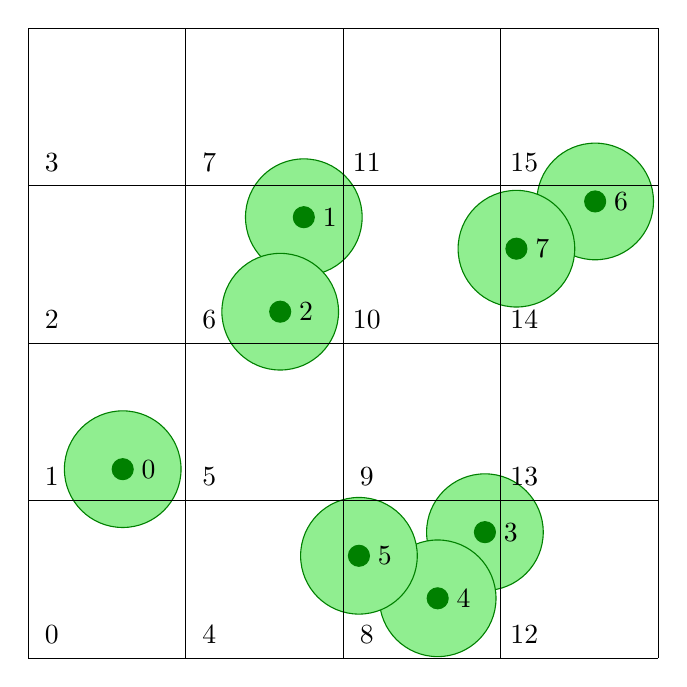
\begin{tikzpicture} 
            \pgfmathsetmacro\dx{2};
            \pgfmathsetmacro\radius{\dx / 2.7};
            \pgfmathsetmacro\centerRadius{\dx / 15};

            \pgfmathsetmacro\x{0.6*\dx};
            \pgfmathsetmacro\y{1.2*\dx};
            \filldraw[draw=Green,fill=LightGreen] (\x,\y) circle (\radius);
            \filldraw[draw=Green,fill=Green] (\x,\y) circle (\centerRadius) node[right]{~0};

            \pgfmathsetmacro\x{1.75*\dx};
            \pgfmathsetmacro\y{2.8*\dx};
            \filldraw[draw=Green,fill=LightGreen] (\x,\y) circle (\radius);
            \filldraw[draw=Green,fill=Green] (\x,\y) circle (\centerRadius)node[right]{~1};

            \pgfmathsetmacro\x{1.6*\dx};
            \pgfmathsetmacro\y{2.2*\dx};
            \filldraw[draw=Green,fill=LightGreen] (\x,\y) circle (\radius);
            \filldraw[draw=Green,fill=Green] (\x,\y) circle (\centerRadius)node[right]{~2};

            \pgfmathsetmacro\x{2.9*\dx};
            \pgfmathsetmacro\y{0.8*\dx};
            \filldraw[draw=Green,fill=LightGreen] (\x,\y) circle (\radius);
            \filldraw[draw=Green,fill=Green] (\x,\y) circle (\centerRadius)node[right]{~3};

            \pgfmathsetmacro\x{2.6*\dx};
            \pgfmathsetmacro\y{0.38*\dx};
            \filldraw[draw=Green,fill=LightGreen] (\x,\y) circle (\radius);
            \filldraw[draw=Green,fill=Green] (\x,\y) circle (\centerRadius)node[right]{~4};

            \pgfmathsetmacro\x{2.1*\dx};
            \pgfmathsetmacro\y{0.65*\dx};
            \filldraw[draw=Green,fill=LightGreen] (\x,\y) circle (\radius);
            \filldraw[draw=Green,fill=Green] (\x,\y) circle (\centerRadius)node[right]{~5};

            \pgfmathsetmacro\x{3.6*\dx};
            \pgfmathsetmacro\y{2.9*\dx};
            \filldraw[draw=Green,fill=LightGreen] (\x,\y) circle (\radius);
            \filldraw[draw=Green,fill=Green] (\x,\y) circle (\centerRadius)node[right]{~6};

            \pgfmathsetmacro\x{3.1*\dx};
            \pgfmathsetmacro\y{2.6*\dx};
            \filldraw[draw=Green,fill=LightGreen] (\x,\y) circle (\radius);
            \filldraw[draw=Green,fill=Green] (\x,\y) circle (\centerRadius)node[right]{~7};

            

            \foreach \x in {0,1,2,3}{
                \foreach \y in {0,1,2,3}{  
                    \draw (\x*\dx,\y*\dx) -- (\x*\dx+\dx,\y*\dx);
                    \draw (\x*\dx,\y*\dx) -- (\x*\dx,\y*\dx+\dx);
                    \draw (\x*\dx+\dx,\y*\dx) -- (\x*\dx+\dx,\y*\dx+\dx);
                    \draw (\x*\dx,\y*\dx+\dx) -- (\x*\dx+\dx,\y*\dx+\dx);
                    \pgfmathtruncatemacro\result{\x*4 + \y};
                    \node at (\x*\dx+0.3,\y*\dx+0.3) {\result};
                }
            }

            

            
        \end{tikzpicture}
        \subcaption{The indices and positions of the particles, after they are sorted according to their hashes, in step 3.}
    \end{minipage}%
    \begin{minipage}[t]{.43\linewidth}
        \vspace{0pt}
        \centering
        \begin{tabular}{|c | c | c|} 
            \hline
            cell & $cellStart$ & $cellEnd$ \\ [0.5ex] 
            \hline\hline
            0 & ~ & ~ \\ 
            \hline
            1 & 0 & 0 \\ 
            \hline
            2 & ~ & ~ \\ 
            \hline
            3 & ~ & ~ \\ 
            \hline
            4 & ~ & ~ \\ 
            \hline
            5 & ~ & ~ \\ 
            \hline
            6 & 1 & 2 \\ 
            \hline
            7 & ~ & ~ \\ 
            \hline
            8 & 3 & 5 \\ 
            \hline
            9 & ~ & ~ \\ 
            \hline
            10 & ~ & ~ \\ 
            \hline
            11 & ~ & ~ \\ 
            \hline
            12 & ~ & ~ \\ 
            \hline
            13 & ~ & ~ \\ 
            \hline
            14 & 6 & 7 \\ 
            \hline
            15 & ~ & ~ \\ 
            \hline

            
        \end{tabular}
        \subcaption{The final result of spatial indexing, represented as the $cellStart$ and $cellEnd$ array.}
    \end{minipage}%

    \caption{Example of spatial indexing in 2D}
    \label{figure spatial indexing}
\end{figure}


\begin{enumerate}
    \item Decide on a hash function for 3D grid coordinates. For example, in an $N*N*N$ grid, the hash of the coordinate $(x,y,z)$ can be $xN^2+yN+z$, which fully avoids hash collision.
    
    \item Create an array of hashes for particles. For each particle, use its physical position to compute the cell that it is in, and compute the hash of that cell as the hash of the particle. Store the hashes of all particles in this array. Since these steps is independent for each particle, it can be efficiently parallelized.
    
    \item Sort this array of particle hashes, and sort the array of particles into the same order. 
    
    \item Create two arrays $cellStart$ and $cellEnd$, which denote, for each cell, the first and the last particle inside the cell. To compute elements of these arrays, for the $i$th particle, use the hash array to check if the $i-1$th particle is in the same cell, if not, the $cellStart$ of this cell should be $i$. Similarly, if the $i+1$th particle is not in the same cell, the $cellEnd$ of this cell should be $i$. This can also be done for all particles in parallel.
    
\end{enumerate}
Having created the $cellStart$ and $cellEnd$ arrays, for each cell, the particles inside it is them simply the particles with index $\geq cellStart$ and $\leq cellEnd$. A 2D example of this procedure is illustrated in figure \ref{figure spatial indexing}.

With all other steps being completely parallelizable, the only complicated step is sorting the array of particle hashes. The implementation of this project uses the thoroughly optimized sorting library provided with the CUDA API. The resulting cost of the spatial indexing is almost negligible compared to other tasks, such as solving systems of linear equations.



\subsection{Jacobi Linear Solver}
The two linear systems to be solved in each simulation step, the Poisson pressure equation and the diffusion equation, both have the special property of being \textit{symmetric positive-definite}. Many advanced approaches have been proposed on how to solve these types of matrices, such as ICPCG \cite{bridson2015fluid} and \textit{Geometric Multigrid}\cite{chentanez2011real}. This project chooses to implement a simpler algorithm, called the Jacobi solver. Though not as fast as the most advanced methods, its efficiency and accuracy is found to be sufficient for the real time simulations in this project.

In the Jacobi Solver, given a system of linear equations written in matrix form:
$$
A\textbf{x}=\textbf{b}
$$
the matrix $A$ is decomposed into $D+C$, where $D$ is a diagonal matrix, and $C$ has only $0$s on the diagonal:
$$
(D+C)\textbf{x}=\textbf{b}
$$
The system is then rewritten as 
$$
D\textbf{x}=\textbf{b} - C\textbf{x}
$$
Thus,
$$
\textbf{x}=D^{-1}(\textbf{b} - C\textbf{x})
$$
which motives an iterative scheme: begin with an initial guess $\textbf{x}_0$, and then iteratively compute
$$
\textbf{x}_{i+1} = D^{-1}(\textbf{b} - C\textbf{x}_{i})
$$
For a certain amount of iterations. Each iterations is simple to do, because $D$ is only a diagonal matrix. 


\subsection{Results}
Performances of the FLIP algorithm implemented in this project highly depend on the simulation parameters used. For a grid of size $50^3$, approximately 100 Jacobi iterations are required at each time step to ensure incompressibility. And with roughly 8 particles inside each grid cell, the simulation alone (without rendering) runs at over 50 FPS(frames per second), which comfortably meets the requirements of real time applications. With rendering added, the frame rate drops to around 20FPS, which is caused by the rather expensive volume rendering(section \ref{subsection multiphase render}) and surface reconstruction(section \ref{section surface reconstruction}). Screenshots of some example simulations follow below.
\begin{figure}[H]
    \centering
    
    \begin{minipage}[t]{.42\linewidth}
        \centering
        \vspace{0pt}
        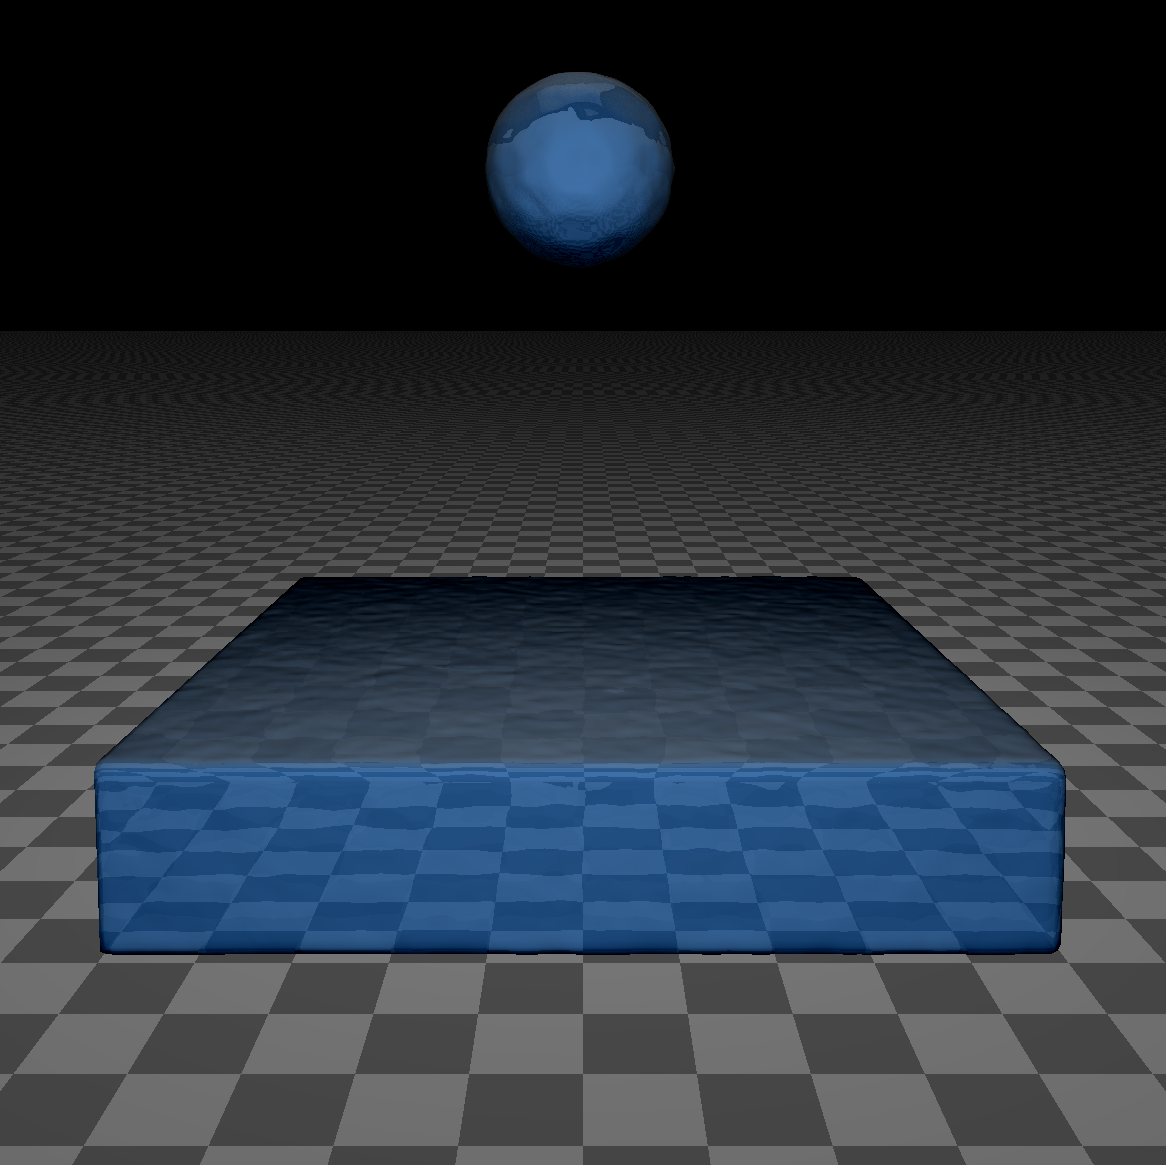
\includegraphics[width=6cm]{balldrop_cropped2/single0.png}
    \end{minipage}
    \begin{minipage}[t]{.42\linewidth}
        \centering
        \vspace{0pt}
        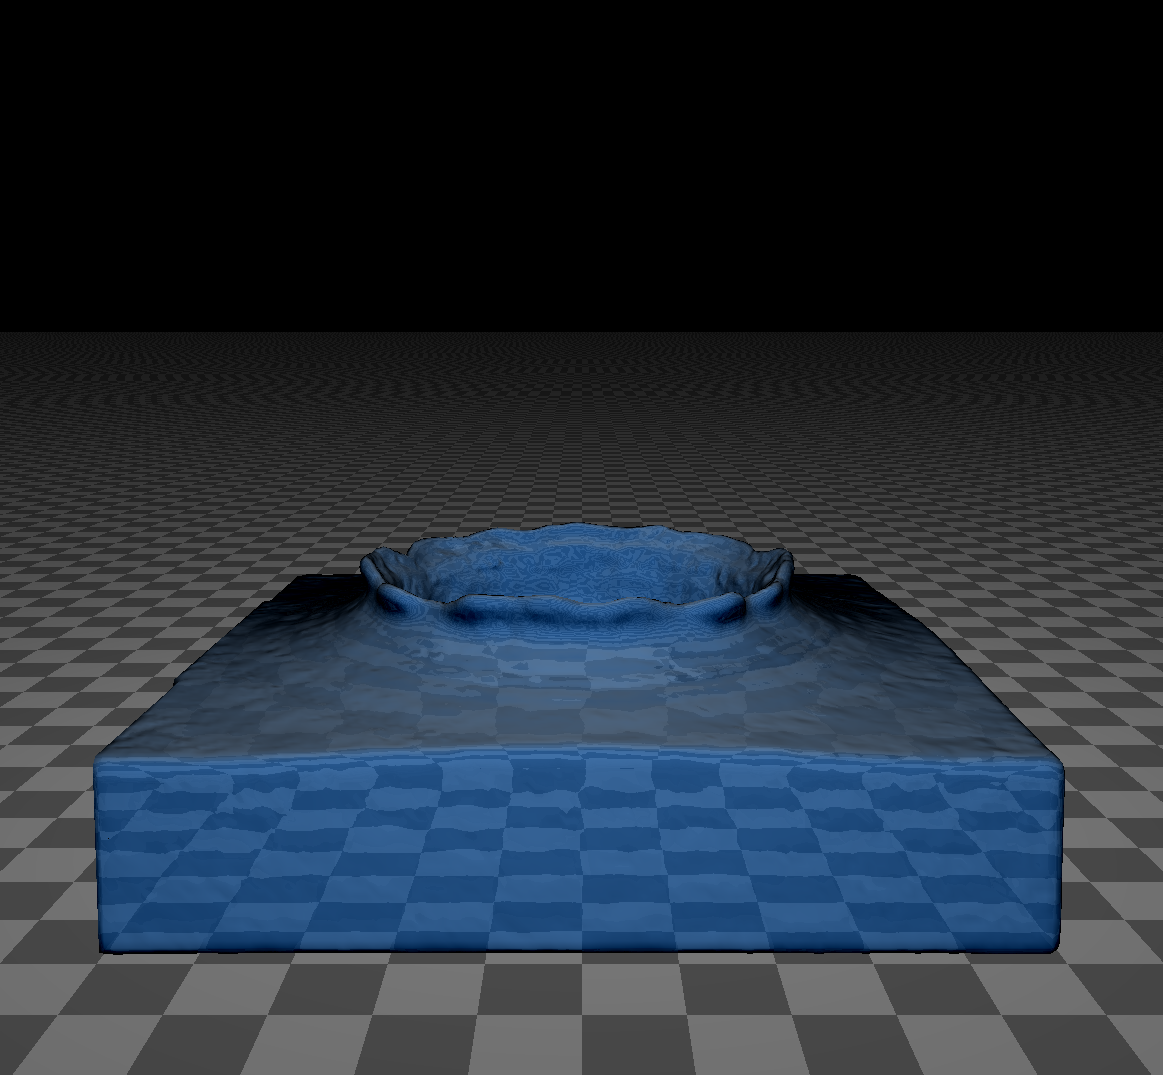
\includegraphics[width=6cm]{balldrop_cropped2/single1.png}
    \end{minipage}

    \vspace{0.5cm}

    \begin{minipage}[t]{.42\linewidth}
        \centering
        \vspace{0pt}
        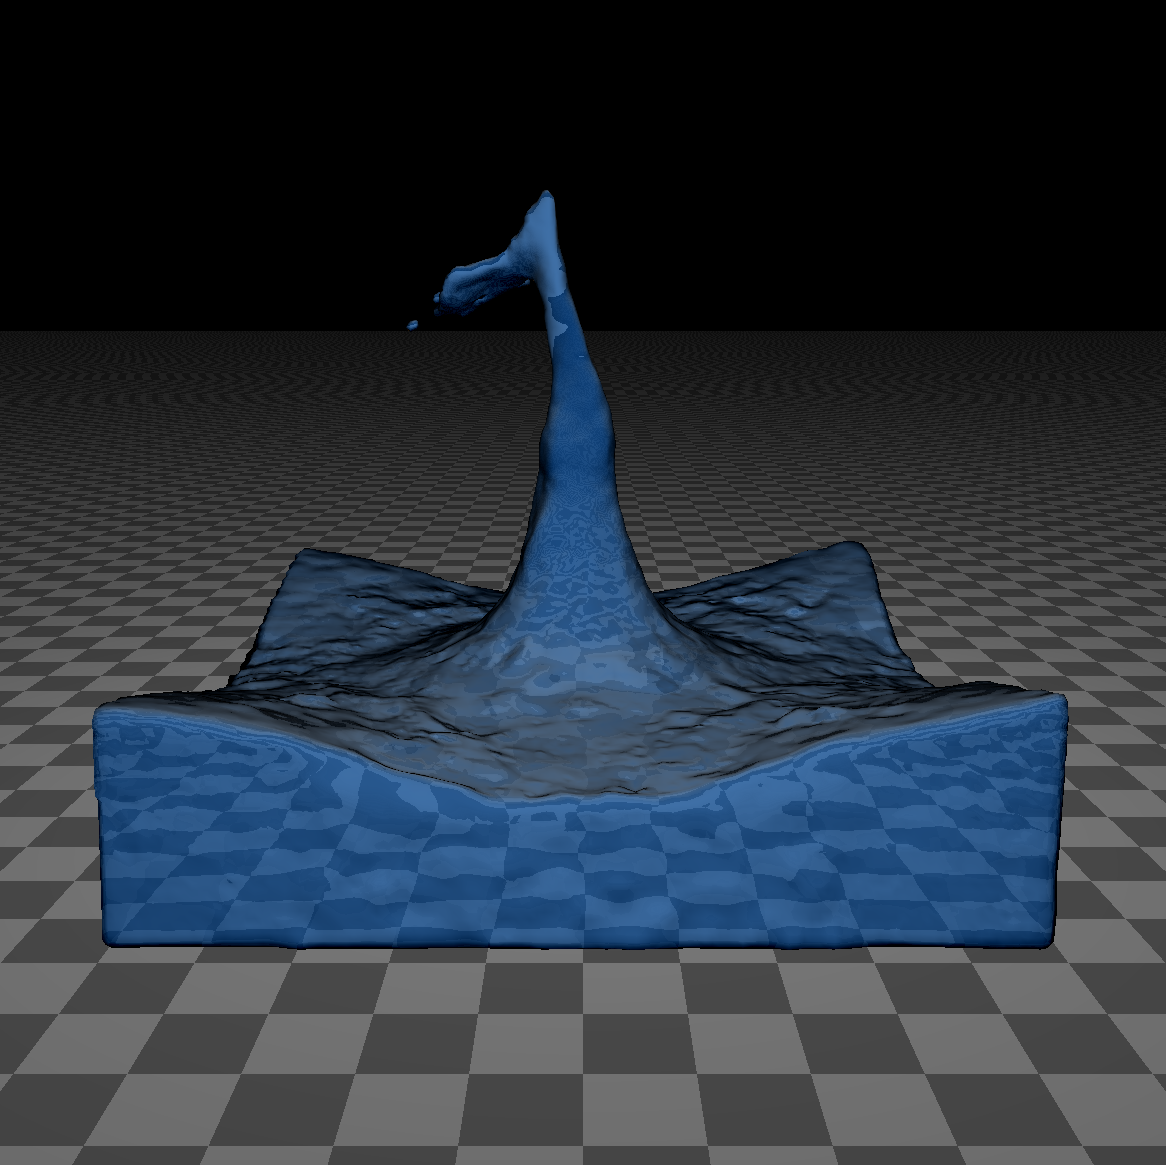
\includegraphics[width=6cm]{balldrop_cropped2/single2.png}
    \end{minipage}
    \begin{minipage}[t]{.42\linewidth}
        \centering
        \vspace{0pt}
        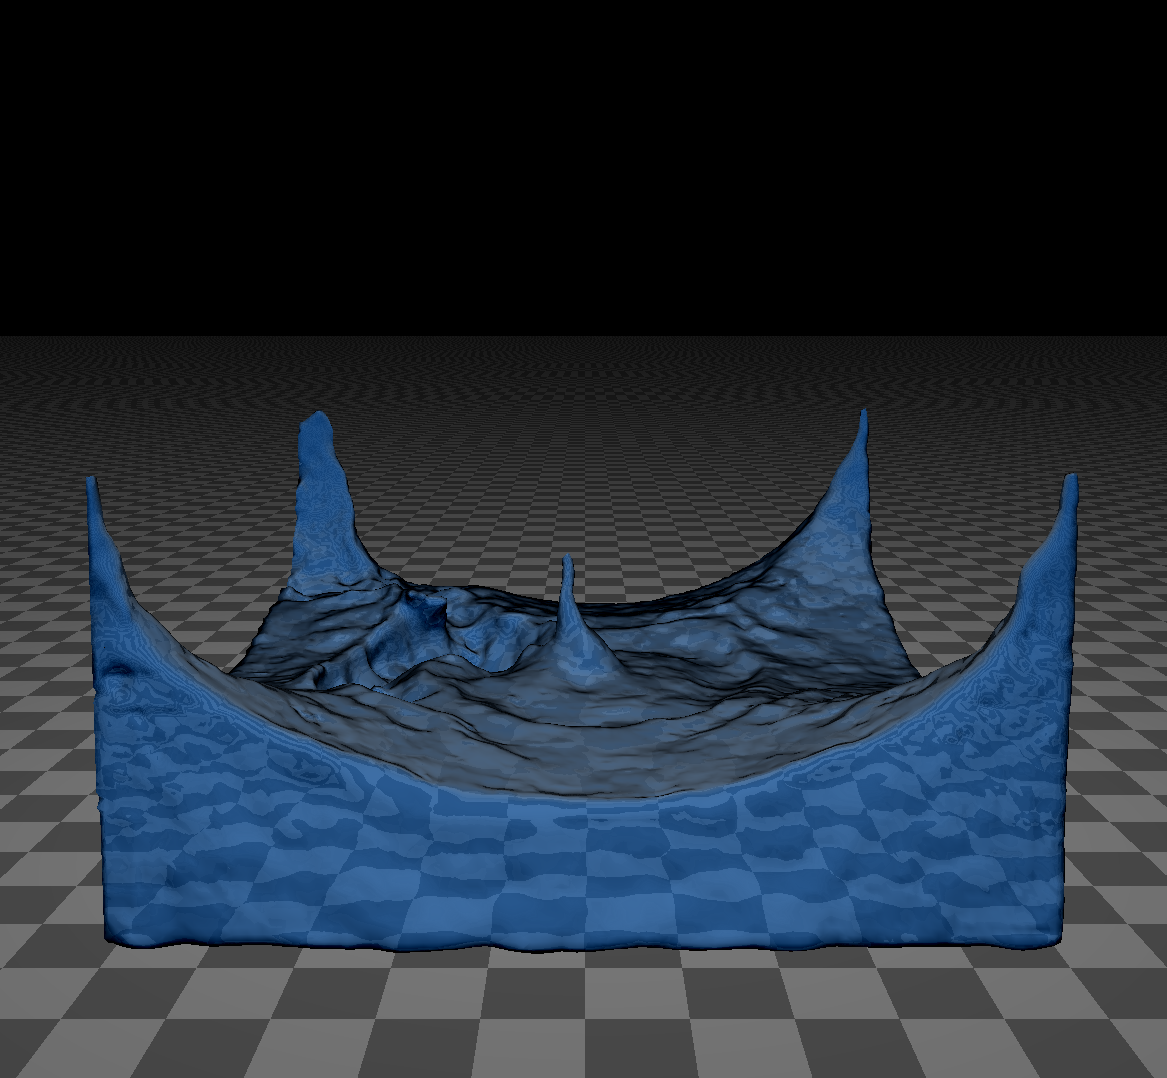
\includegraphics[width=6cm]{balldrop_cropped2/single3.png}
    \end{minipage}

    \caption{Ball drop. $50^3$ grid, $208k$ FLIP particles}
    \label{figure ball drop single}
\end{figure}


\begin{figure}[H]
    \centering
    
    \begin{minipage}[t]{.42\linewidth}
        \centering
        \vspace{0pt}
        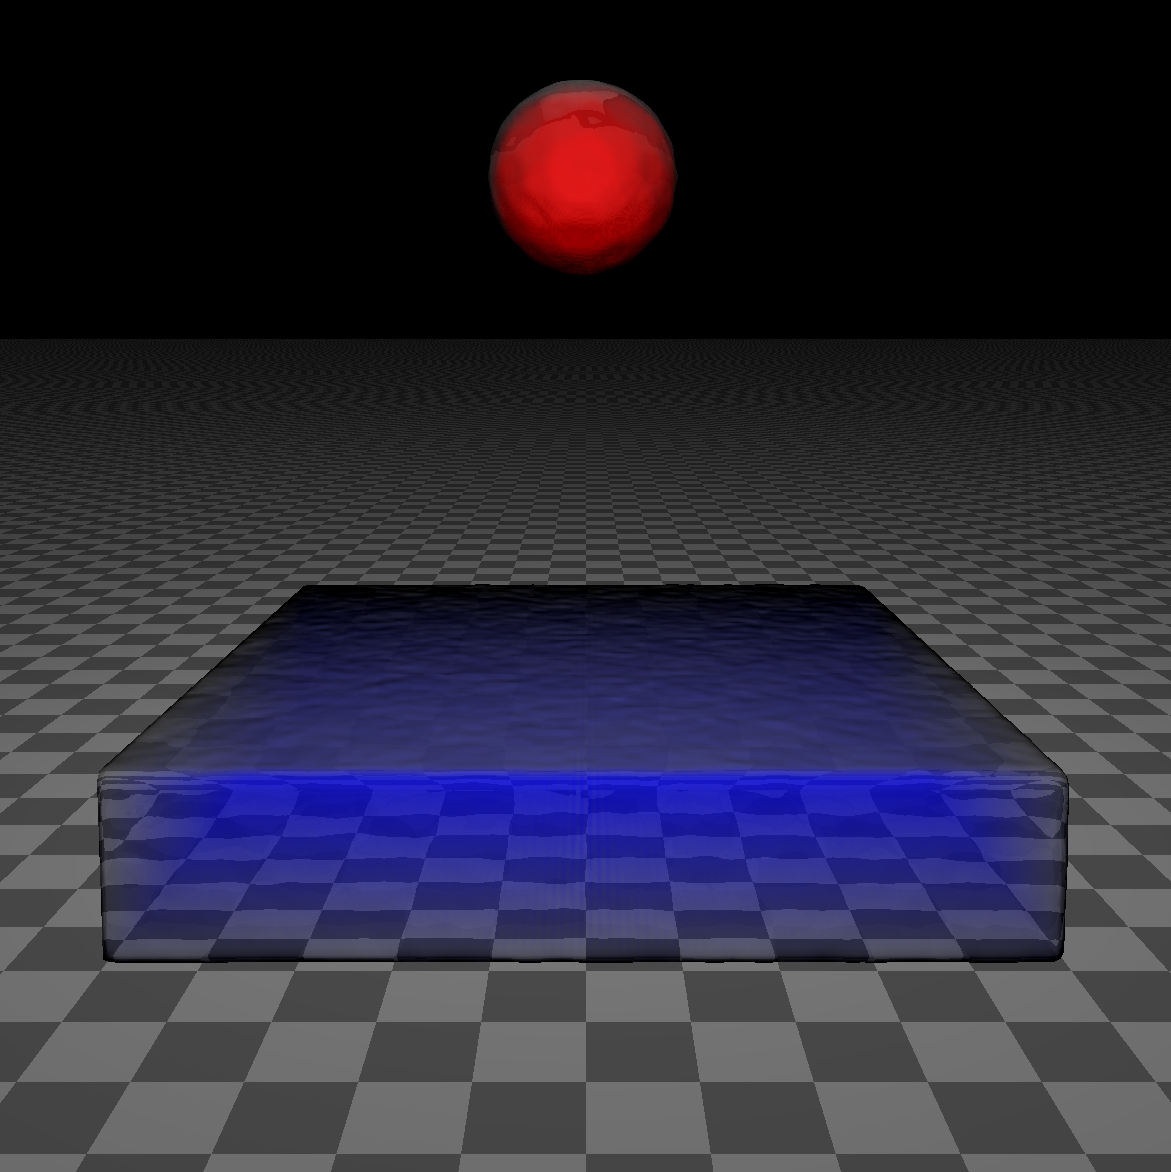
\includegraphics[width=6cm]{balldrop_cropped2/multi0.png}
    \end{minipage}
    \begin{minipage}[t]{.42\linewidth}
        \centering
        \vspace{0pt}
        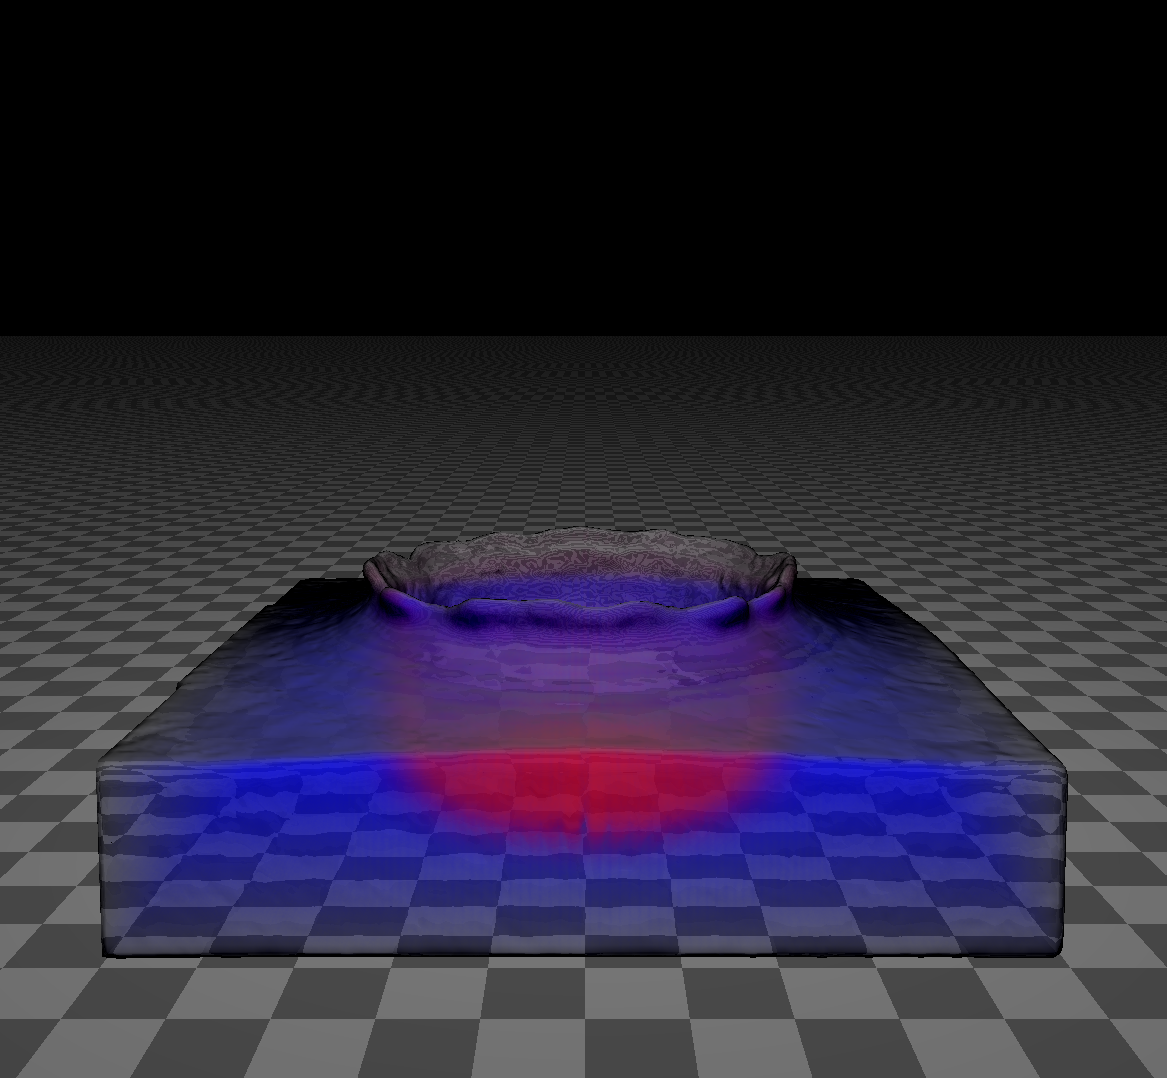
\includegraphics[width=6cm]{balldrop_cropped2/multi1.png}
    \end{minipage}

    \vspace{0.5cm}

    \begin{minipage}[t]{.42\linewidth}
        \centering
        \vspace{0pt}
        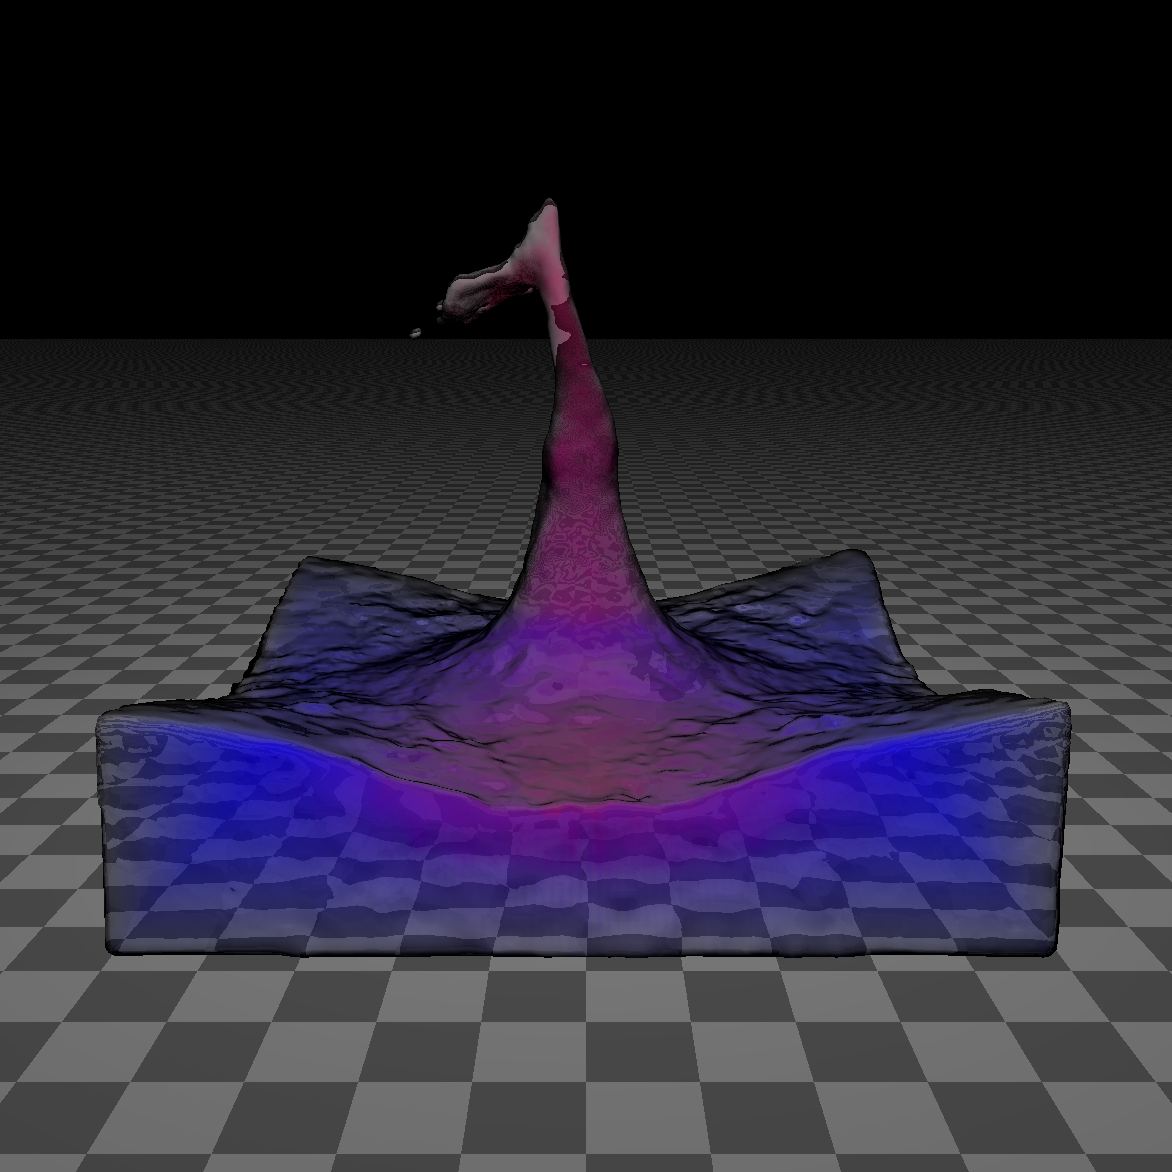
\includegraphics[width=6cm]{balldrop_cropped2/multi2.png}
    \end{minipage}
    \begin{minipage}[t]{.42\linewidth}
        \centering
        \vspace{0pt}
        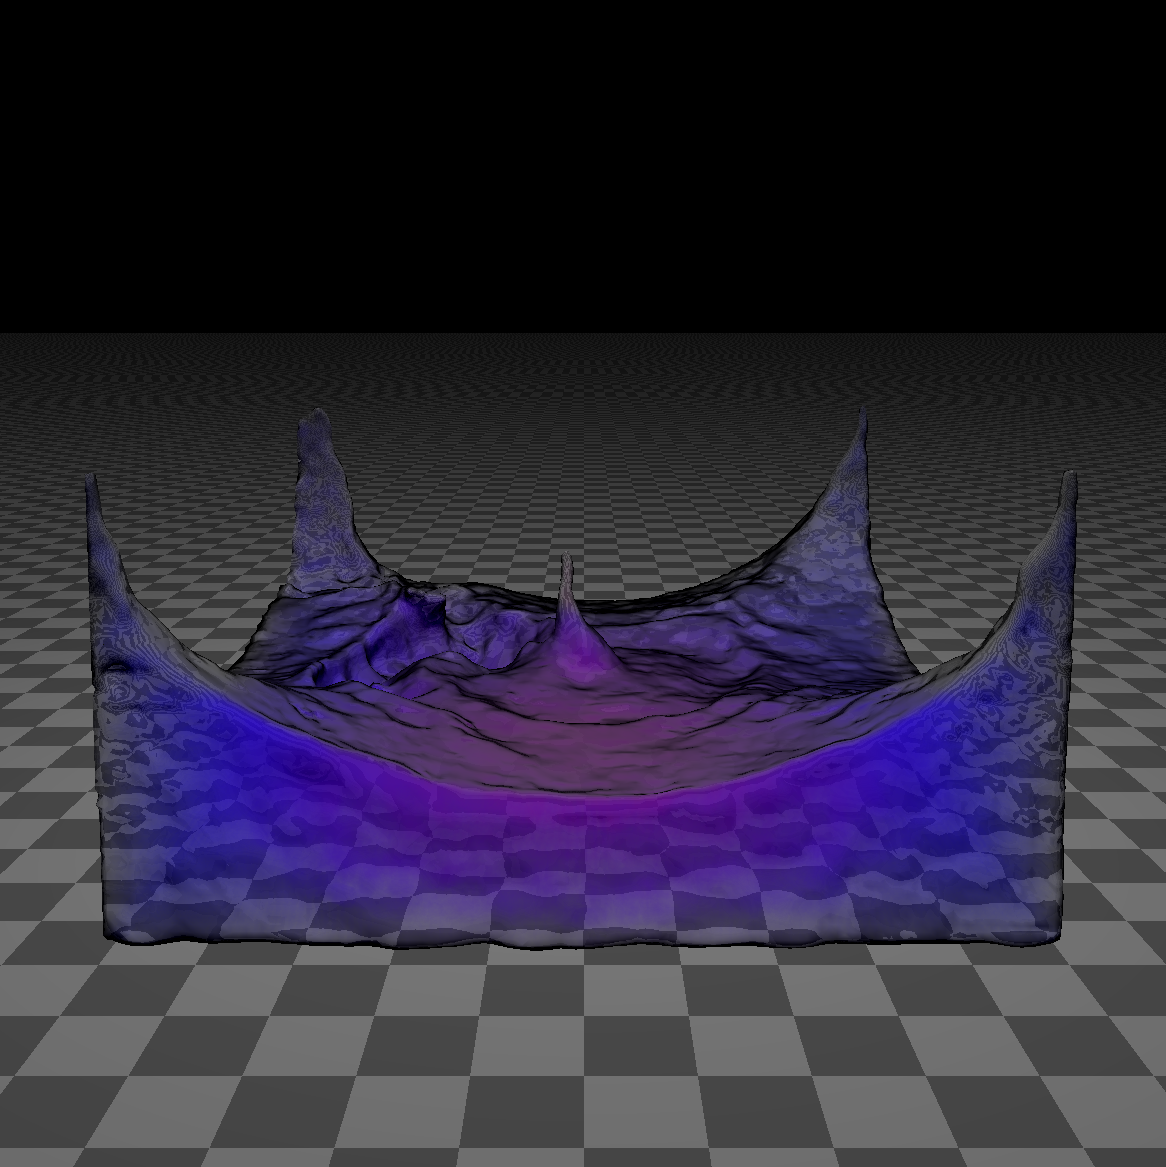
\includegraphics[width=6cm]{balldrop_cropped2/multi3.png}
    \end{minipage}

    \caption{Same simulation as figure \ref{figure ball drop single}, except with 2 phases}
    \label{figure ball drop multi}
\end{figure}


\begin{figure}[H]
    \centering
    
    \begin{minipage}[t]{.24\linewidth}
        \centering
        \vspace{0pt}
        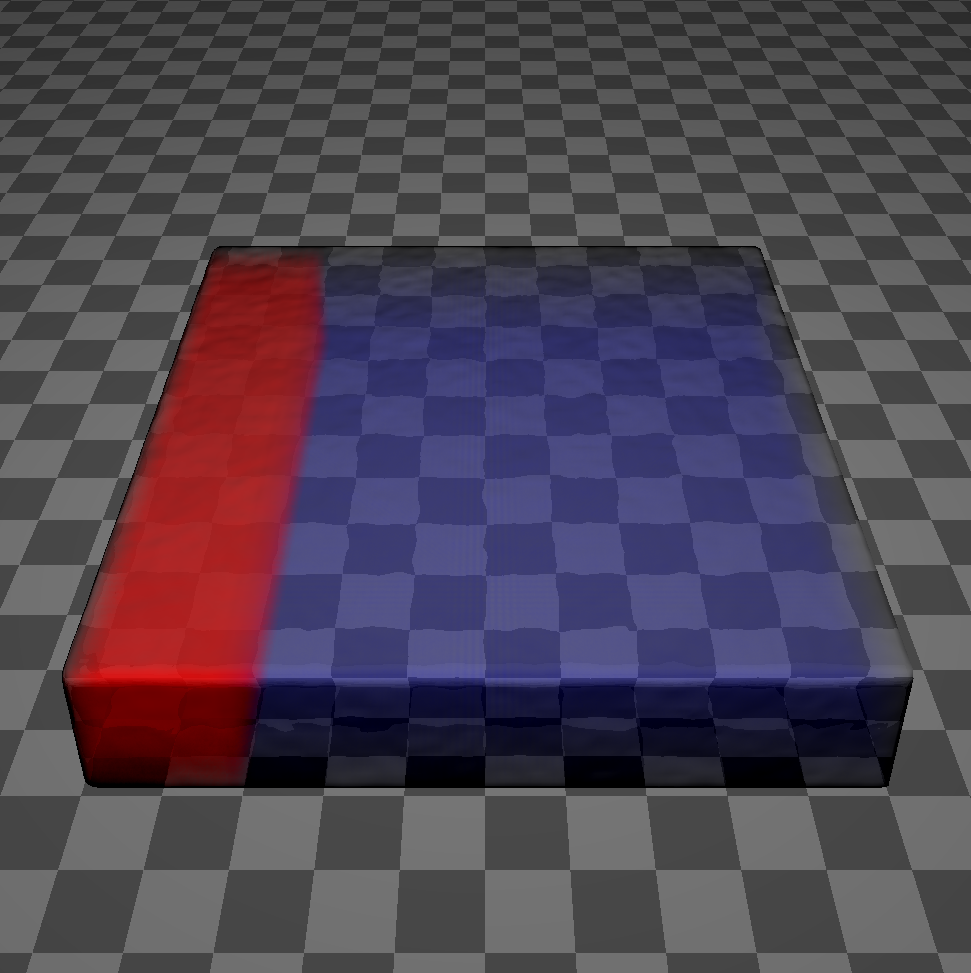
\includegraphics[width=3.5cm]{diffusion_cropped/small0.png}
    \end{minipage}
    \begin{minipage}[t]{.24\linewidth}
        \centering
        \vspace{0pt}
        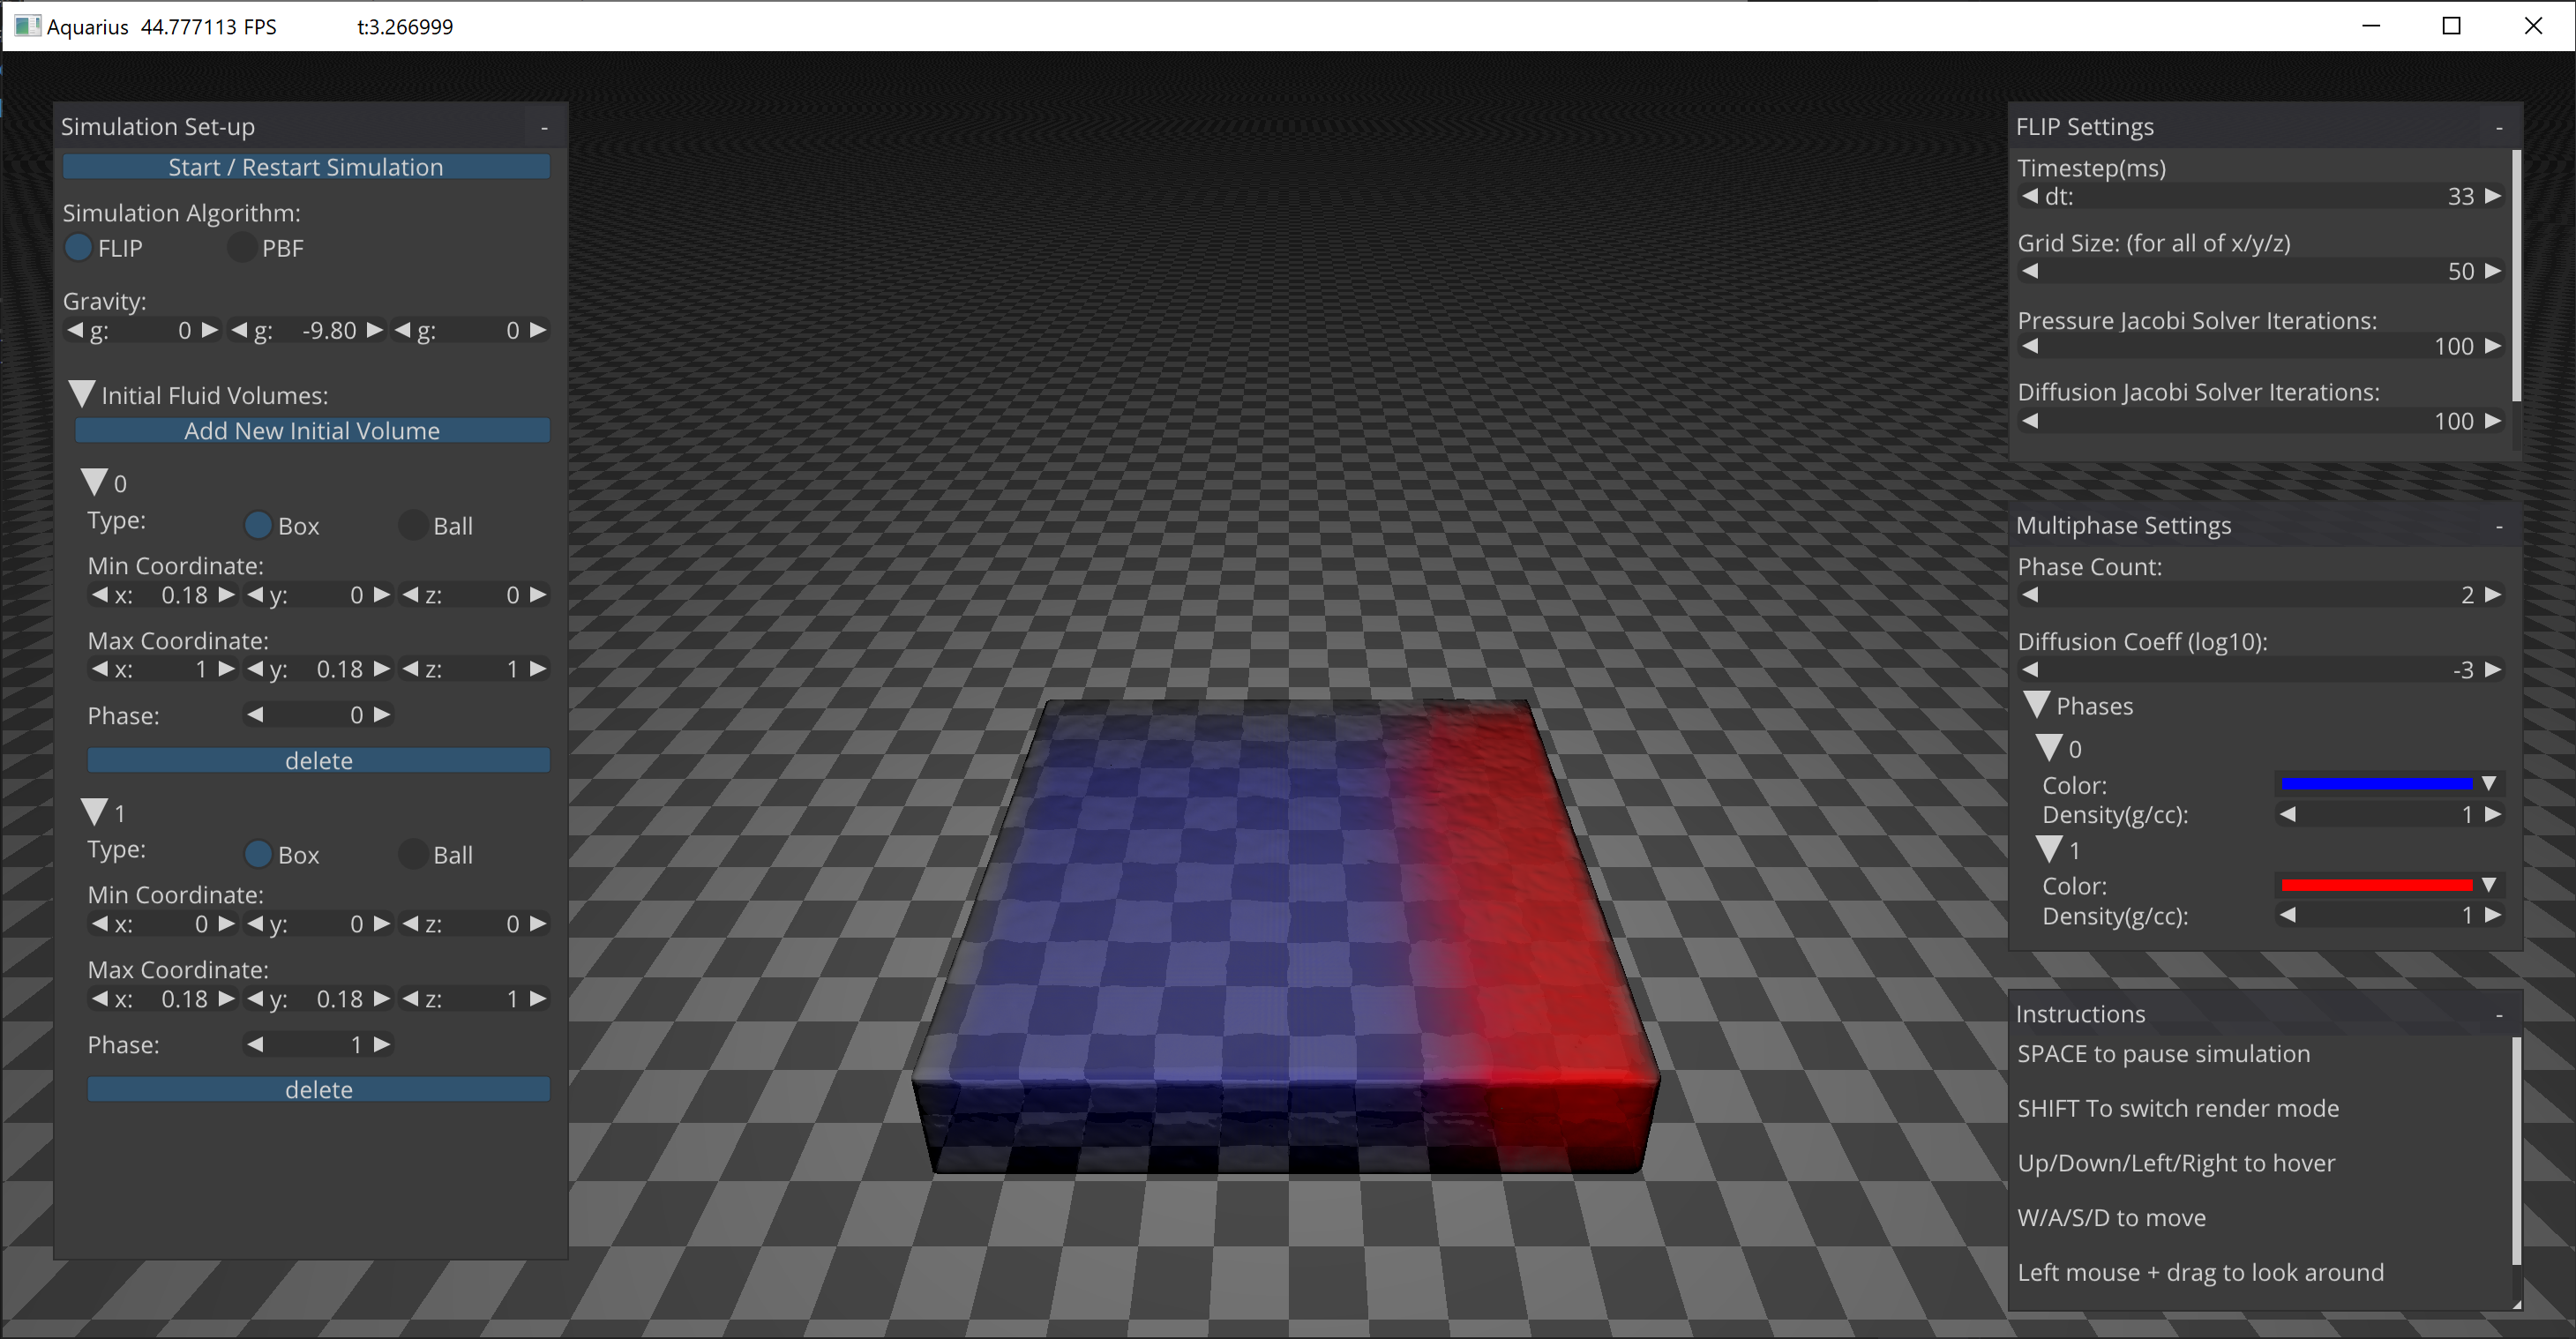
\includegraphics[width=3.5cm]{diffusion_cropped/small1.png}
    \end{minipage}
    \begin{minipage}[t]{.24\linewidth}
        \centering
        \vspace{0pt}
        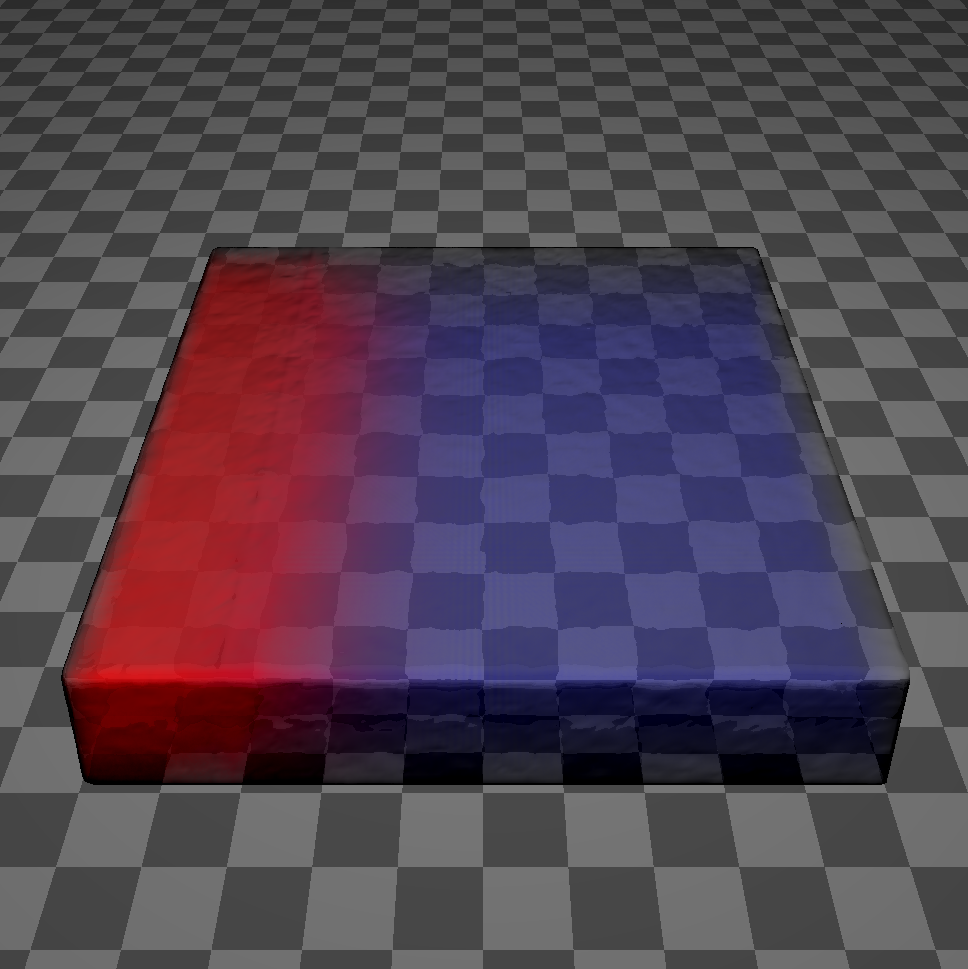
\includegraphics[width=3.5cm]{diffusion_cropped/small2.png}
    \end{minipage}
    \begin{minipage}[t]{.24\linewidth}
        \centering
        \vspace{0pt}
        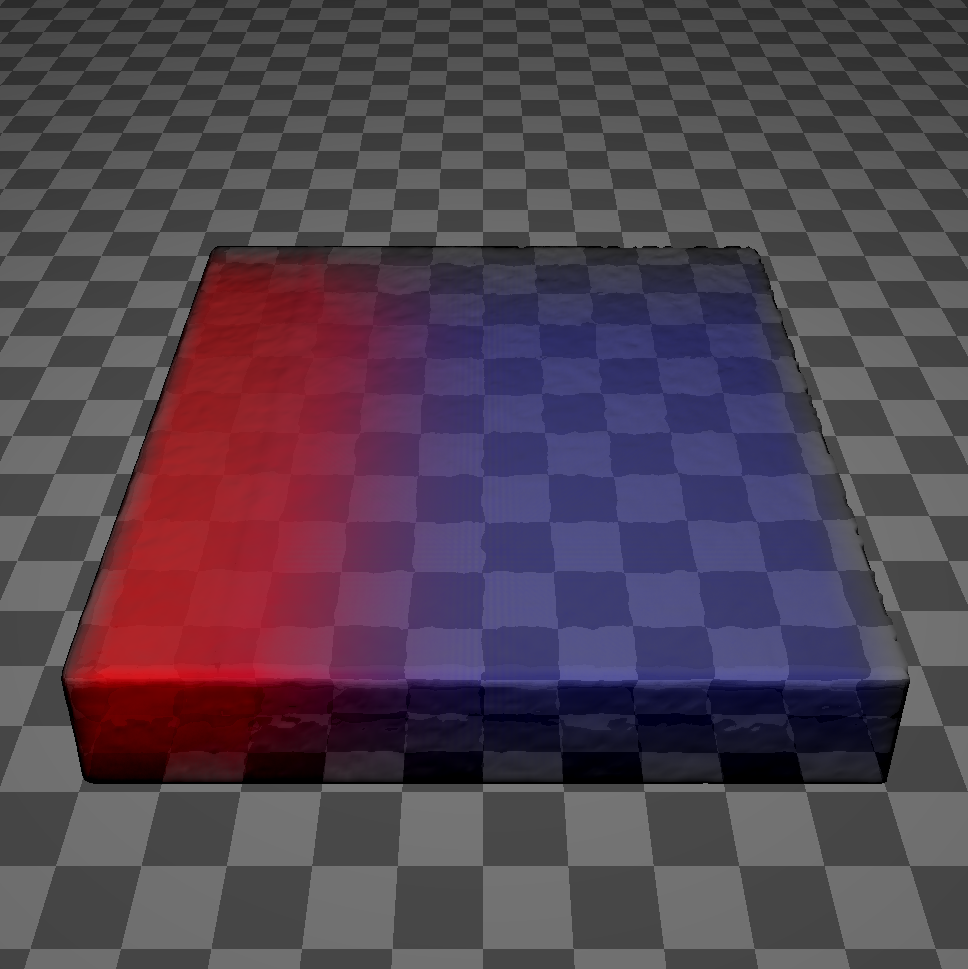
\includegraphics[width=3.5cm]{diffusion_cropped/small3.png}
    \end{minipage}

    \caption{Diffusion with coefficient $10^{-3}$}
    \label{diffusion 1e-3}
\end{figure}



\begin{figure}[H]
    \centering
    
    \begin{minipage}[t]{.24\linewidth}
        \centering
        \vspace{0pt}
        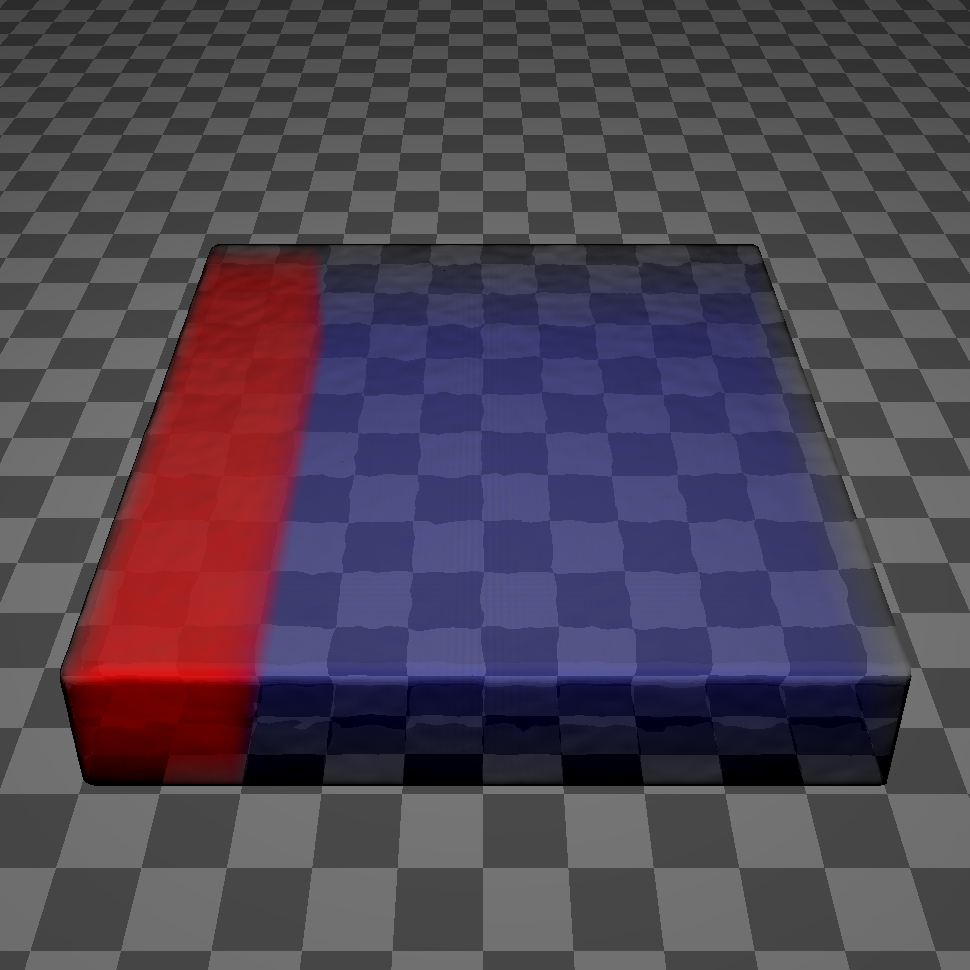
\includegraphics[width=3.5cm]{diffusion_cropped/big0.png}
    \end{minipage}
    \begin{minipage}[t]{.24\linewidth}
        \centering
        \vspace{0pt}
        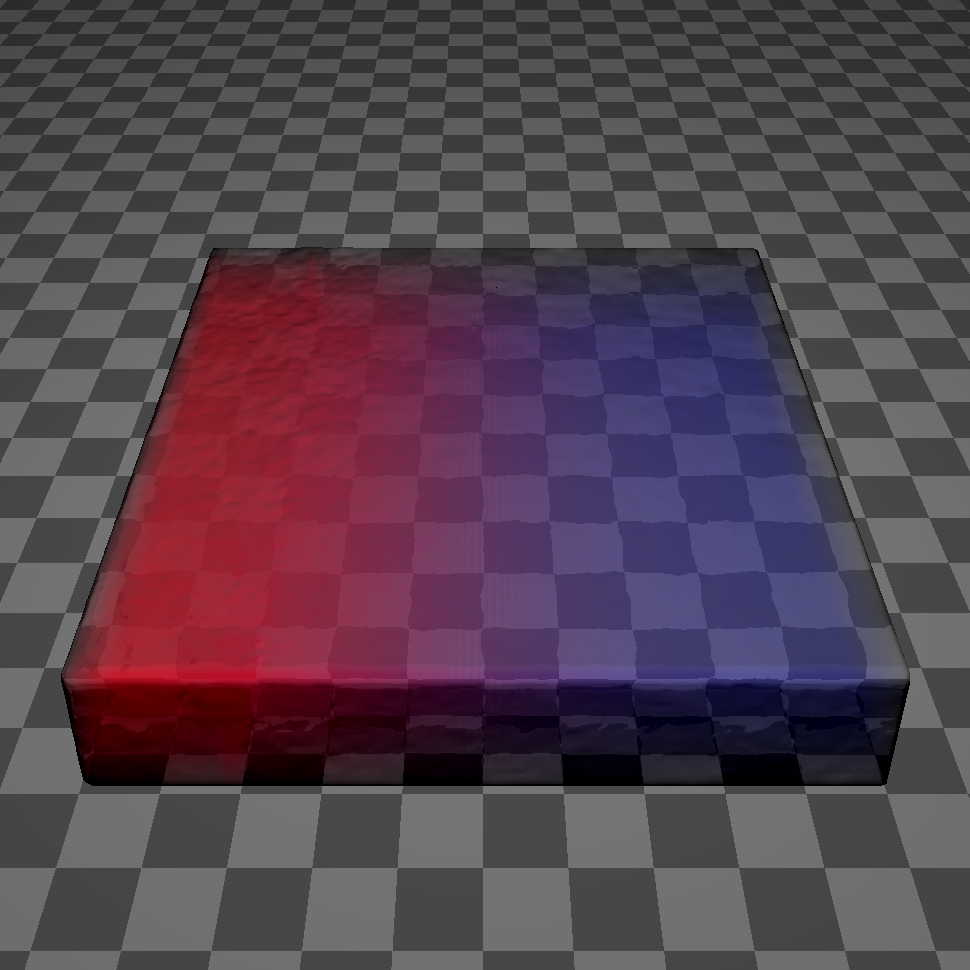
\includegraphics[width=3.5cm]{diffusion_cropped/big1.png}
    \end{minipage}
    \begin{minipage}[t]{.24\linewidth}
        \centering
        \vspace{0pt}
        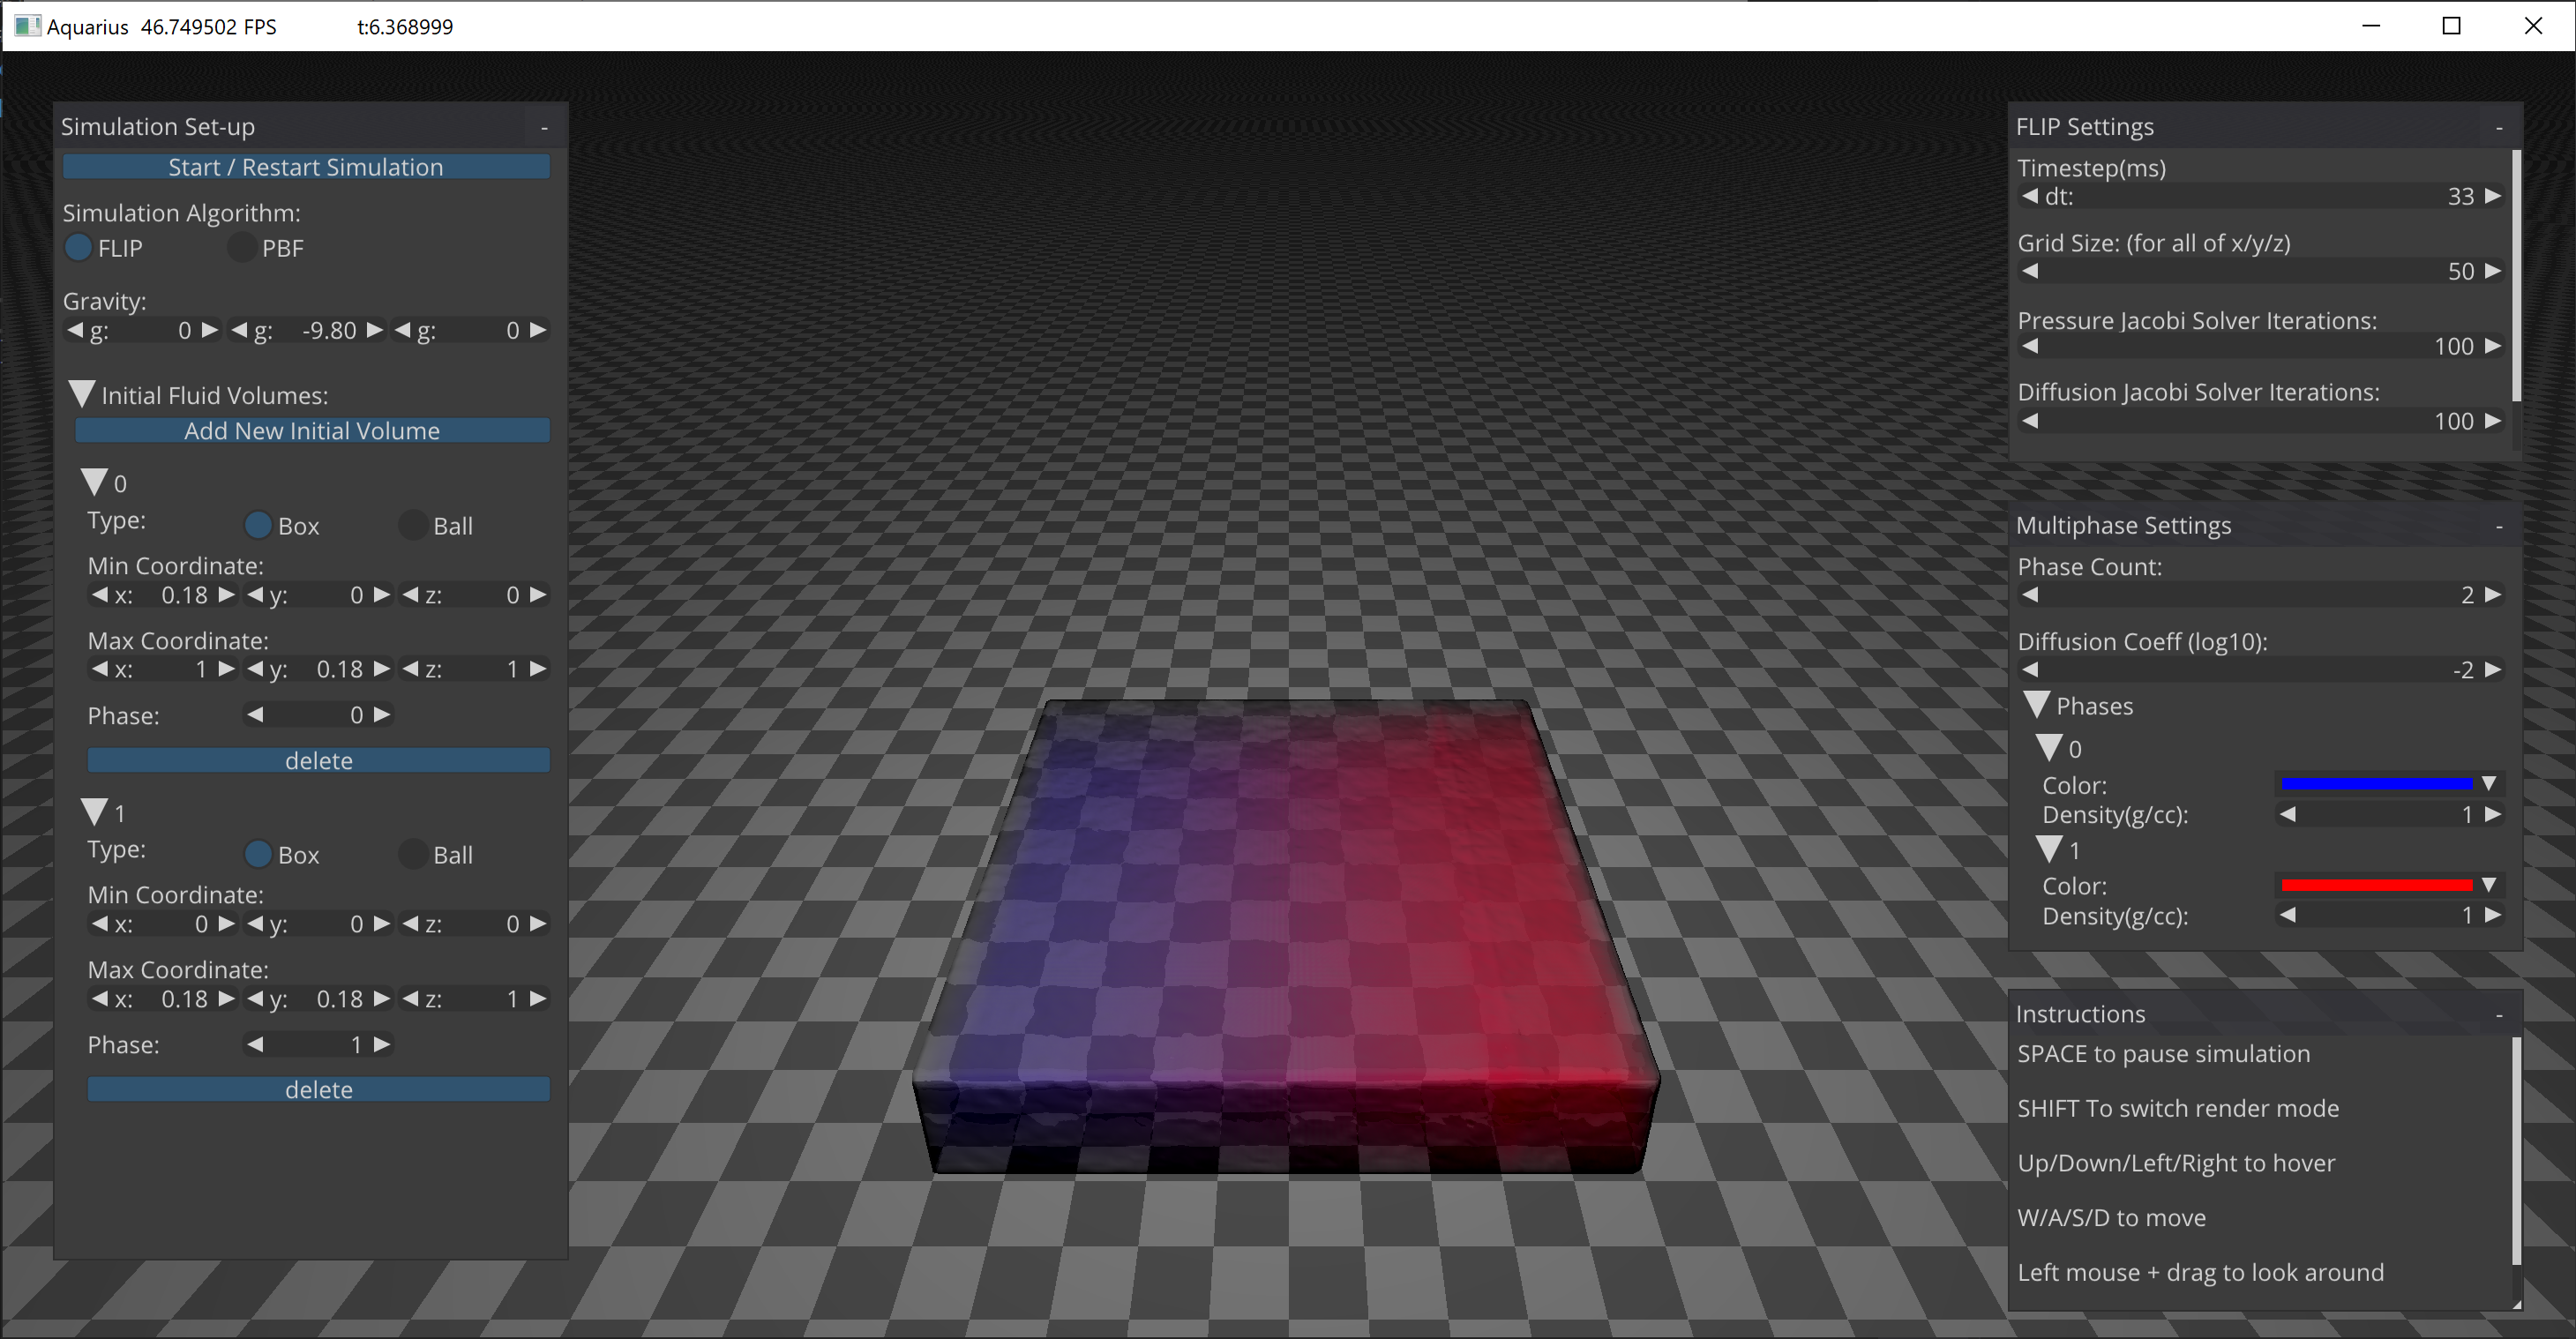
\includegraphics[width=3.5cm]{diffusion_cropped/big2.png}
    \end{minipage}
    \begin{minipage}[t]{.24\linewidth}
        \centering
        \vspace{0pt}
        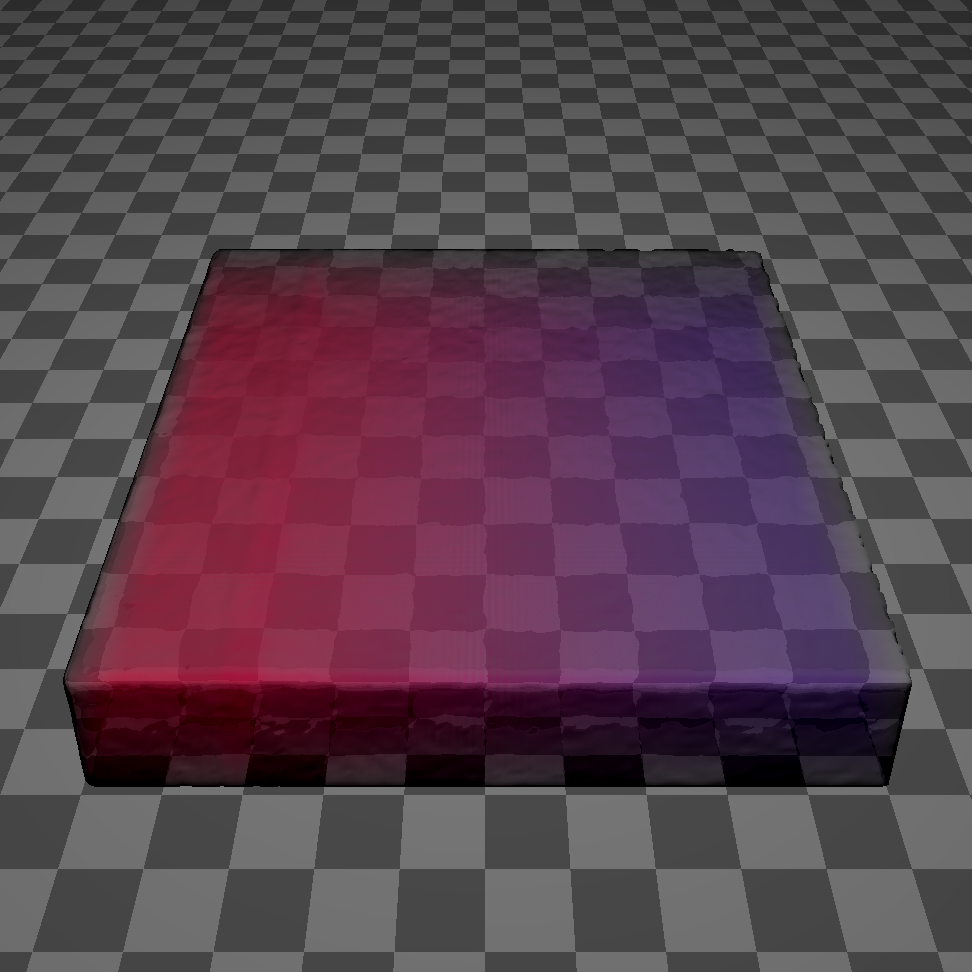
\includegraphics[width=3.5cm]{diffusion_cropped/big3.png}
    \end{minipage}

    \caption{Diffusion with coefficient $10^{-2}$}
    \label{diffusion 1e-2}
\end{figure}



\chapter{Particle-Based Simulations}
\label{chapter particle}



Besides the grid-based fluid simulations algorithms, this project also studied and implemented a fundamentally different algorithm, known as \textbf{PBF} (Position-Based Fluids), which only uses particles to represent the fluid and its relevant scalar and vector fields. This chapter explains the principles of this algorithm, its CUDA implementation, and how it compares to the FLIP algorithm presented in the last chapter.

\section{Smoothed Particle Hydrodynamics}
PBF belongs to a family of algorithms called \textit{Smoothed Particle Hydrodynamics}, or SPH. Similar to FLIP, SPH algorithms represent the fluid using a cloud of particles. All quantities that are involved in the simulations are carried by the particles. For some quantity $q$, either scalar or vector, and some location $\textbf{x}$, SPH approximates $q$ at $q(\textbf{x})$ as a weighted average of $Q$ carried by the nearby particles.
\begin{equation}
    \label{eqn SPH basic}
    \begin{aligned}
        Q(\textbf{x}) = \sum_{j=1}^N m_j \frac{Q_j}{\rho_j} W(\textbf{x}-\textbf{x}_j,h)
    \end{aligned}
\end{equation}
where $N$ is the total amount of particles, $m_j$ is the mass of the $j$th particle, $\textbf{x}_j$ its position, $\rho_j$ its density, and $Q_j$ the value of $Q$ it carries. Most importantly, $W$ is a \textit{smoothing kernel function}, and $h$ its \textit{smoothing radius}, which satisfies the properties:
\begin{equation}
    \begin{aligned}
        \forall\textbf{r}~~s.t~~||\textbf{r}||>h, W(\textbf{r},h) &= 0\\
        \int W(\textbf{r},h) d\textbf{r} &= 1
    \end{aligned}
\end{equation}
$W$ is used to decide the contribution weight of each particle, which is greater if $\textbf{x}_j$ is closer to $\textbf{x}$. Thus, normally the value of $W(\textbf{r},h)$ only depends on $||r||$, and is $0$ if $||r||>h$.


A convenient and important property of the SPH framework is that, computing the gradient/Laplacian of a quantity can be done by only applying the gradient/Laplacian operator on the smoothing kernel:
\begin{equation}
    \label{eqn SPH derivative}
    \begin{aligned}
        \nabla Q(\textbf{x}) &= \sum_{j} m_j \frac{Q_j}{\rho_j} \nabla W(\textbf{x}-\textbf{x}_j,h) \\
        \nabla \cdot \nabla Q(\textbf{x}) &= \sum_{j} m_j \frac{Q_j}{\rho_j} \nabla \cdot \nabla W(\textbf{x}-\textbf{x}_j,h)
    \end{aligned}
\end{equation}
A common choice of $W$ is the ``poly6" function:
$$
    W_{poly6}(\textbf{r},h)=
        \begin{cases}
            \frac{315}{64\pi h^9}(h^2-||\textbf{r}||^2)^3 &\mbox{ if } 0\leq||\textbf{r}||\leq h\\
            0 &\mbox{otherwise} 
        \end{cases}
$$
However, this function has the problem that, its gradient vanishes as $\textbf{r}$ approaches $\textbf{0}$. Thus, when computing $\nabla W$, a alternative kernel called the ``spiky" kernel is used:
$$
    \nabla W_{spiky}(\textbf{r},h)=
        \begin{cases}
            \frac{-45}{\pi h^6||\textbf{r}||}(h-||\textbf{r}||)^2\textbf{r} &\mbox{ if } 0\leq||\textbf{r}||\leq h\\
            \textbf{0} &\mbox{otherwise} 
        \end{cases}
$$
Figure \ref{figure kernels} illustrates the difference between the two kernels:

\begin{figure}[!h]
    \label{figure kernels}
    \begin{tikzpicture}
        \draw[->] (-3,0) -- (4.2,0) node[right] {$x$};
        \draw[->] (0,-3) -- (0,4.2) node[above] {$y$};
        \draw[scale=1.0,domain=-1:1,smooth,variable=\x,blue,line width=0.25mm] plot ({\x},
           {(1-\x*\x)*(1-\x*\x)*(1-\x*\x)}
        );
        \draw[scale=1.0,domain=-1:1,smooth,variable=\x,red,dashed,line width=0.25mm] plot ({\x},
           {-6*(1-\x*\x)*(1-\x*\x)*\x}
        );
        \draw[blue,line width=0.25mm] (1.5,2.5) -- (2,2.5) node[right] {$W_{poly6}$};
        \draw[red,dashed,line width=0.25mm] (1.5,2) -- (2,2) node[right] {$\nabla W_{poly6}$};
      \end{tikzpicture}
      \begin{tikzpicture}
        \draw[->] (-3,0) -- (4.2,0) node[right] {$x$};
        \draw[->] (0,-3) -- (0,4.2) node[above] {$y$};
        \draw[scale=1.0,domain=-1:1,smooth,variable=\x,blue,line width=0.25mm] plot ({\x},
           {(1-abs(\x))*(1-abs(\x))*(1-abs(\x))}
        );
        \draw[scale=1.0,domain=0:1,smooth,variable=\x,red,dashed,line width=0.25mm] plot ({\x},
           {-3*(1-\x)*(1-\x)}
        );
        \draw[scale=1.0,domain=-1:0,smooth,variable=\x,red,dashed,line width=0.25mm] plot ({\x},
           {3*(1+\x)*(1+\x)}
        );
        \draw[blue,line width=0.25mm] (1.5,2.5) -- (2,2.5) node[right] {$W_{spiky}$};
        \draw[red,dashed,line width=0.25mm] (1.5,2) -- (2,2) node[right] {$\nabla W_{spiky}$};
      \end{tikzpicture}

      \caption{Scalar versions of $W_{poly6}$ and $W_{spiky}$}
      
\end{figure}

In the first paper where SPH is used for computer graphics, written by Matthias Müller\cite{muller2003particle} in 2003, each quantity involved in the Navier-Stokes momentum equation is explicitly written in the forms of formula \ref{eqn SPH basic} or \ref{eqn SPH derivative}. An explicit time stepping integration is then used to update the velocity field and particle positions. However, the incompressibility condition was ignored in that paper. Since then, many extensions and modifications to the original SPH scheme was proposed, which enforces incompressibility. The newest and currently most popular one of these extensions is proposed in 2013, again developed by Müller and his colleague Macklin in NVIDIA\cite{macklin2013position}. This extension is the Position Based Fluids algorithm.


\section{Position Based Fluids}
In Position Based Fluids, or PBF, the incompressibility condition is enforced by putting an explicit constraint on the density of the fluid. To begin with, for each particle $i$ at position $\textbf{x}_i$ the density at each particle can be derived using formula \ref{eqn SPH basic}:
\begin{equation*}
    \begin{aligned}
        \rho_i &= \sum_{j} m_j \frac{\rho_j}{\rho_j} W(\textbf{x}_i-\textbf{x}_j,h)\\
        &= \sum_{j} m_j W(\textbf{x}_i-\textbf{x}_j,h)
    \end{aligned}
\end{equation*}
PBF treats all particles as having equal mass. This mass can be chosen to be $1$, which simplifies the formula:
\begin{equation}
    \label{eqn PBF rho}
    \begin{aligned}
        \rho_i 
        &= \sum_{j} W(\textbf{x}_i-\textbf{x}_j,h)
    \end{aligned}
\end{equation}
Note that $\rho_i$ is in fact a function of the positions of all the particles in the simulation: $\rho_i = \rho_i(\textbf{x}_0,\textbf{x}_1,\dots,\textbf{x}_N)$ where $N$ is the total amount of particles. Using the density of each particle, PBF defines a constraint quantity $C_i$ for each particle $i$:
$$
C_i(\textbf{x}_0,\textbf{x}_1,\dots,\textbf{x}_N) = \frac{\rho_i}{\rho_{rest}} - 1
$$
where $\rho_{rest}$ is the rest density of the fluid. The incompressibility constraint can then be explicitly written as:
$$
C_i(\textbf{x}_0,\textbf{x}_1,\dots,\textbf{x}_N) = 0
$$
Collectively, using the concatenated vector $\textbf{X} = [\textbf{x}_1^T,\textbf{x}_2^T,\dots,\textbf{x}^T]^T$ to denote the positions of all particles, the constraint of the $i$th particle can be written as:
\begin{equation}
    C_i(\textbf{X}) = 0
\end{equation}

In each time step of the PBF simulation, the algorithm begins by predicting a new position $\textbf{x}_i^*$ for each particle $i$ using its velocity $\u_i$:
$$
\textbf{x}_i^* = \textbf{x}_i + \triangle t \u_i
$$
If the particle happens to travel into a solid region, some basic collision handling should also be applied (e.g clamping $\textbf{x}_i^*$ outside the solid).

Let $\textbf{X}^*=[\textbf{x}_1^{*T},\textbf{x}_2^{*T},\dots,\textbf{x}_N^{*T}]^T$ be the collective predicted position, then, in all likelihood, $\textbf{X}^*$ will not satisfy the density constraints. Thus, PBF aims to find a set of corrections for the particles' positions, $\triangle\textbf{X}=[\triangle\textbf{x}_1^T,\triangle\textbf{x}_2^T,\dots,\triangle\textbf{x}_N^T]^T$, which restores the density constraints:
\begin{equation}
    \label{eqn density constrain C(x+dx)=0}
    C_i(\textbf{X}^* + \triangle\textbf{X}) = 0~~\forall i \in [0\dots N]
\end{equation}
PBF approximates $\triangle\textbf{X}$ by restricting it in the direction of $\nabla C_i(\textbf{X}^*)$:
\begin{equation}
    \begin{aligned}
        \triangle\textbf{X} \approx  \lambda_i \nabla C_i(\textbf{X}^*)
    \end{aligned}
\end{equation}
where $\lambda_i$ is a scalar coefficient. To find a suitable $\lambda_i$, PBF considers the 1st order Taylor series of $C_i(\textbf{X}^* + \triangle\textbf{X})$:
\begin{equation}
    \begin{aligned}
        C_i(\textbf{X}^* + \triangle\textbf{X}) 
        &\approx  C_i(\textbf{X}^*) + (\nabla C_i(\textbf{X}^*))^T \triangle\textbf{X} \\
        &\approx  C_i(\textbf{X}^*) + (\nabla C_i(\textbf{X}^*))^T  \nabla C_i(\textbf{X}^*) \lambda_i \\
        &=  C_i(\textbf{X}^*) + ||\nabla C_i(\textbf{X}^*)||^2  \lambda_i
    \end{aligned}
\end{equation}
Combining this with formula \ref{eqn density constrain C(x+dx)=0}, it can be derived that
\begin{equation}
    \label{eqn lambda i basic}
    \begin{aligned}
        \lambda_i &\approx \frac{-C_i(\textbf{X}^*)}{||\nabla C_i(\textbf{X}^*)||^2}\\
        &= \frac{-C_i(\textbf{X}^*)}{ \sum_{j} ||\nabla_{\textbf{x}^*_j} C_i(\textbf{X}^*)||^2}
    \end{aligned}
\end{equation}
The summation in the denominator can be separated into two cases: when $j=i$ and $j\neq i$
\begin{equation}
    \label{eqn lambda i expanded}
    \begin{aligned}
        \lambda_i  \approx\frac{-C_i(\textbf{X}^*)}{ ||\nabla_{\textbf{x}^*_i} C_i(\textbf{X}^*)||^2 + \sum_{j\neq i} ||\nabla_{\textbf{x}^*_j} C_i(\textbf{X}^*)||^2}\\
    \end{aligned}
\end{equation}
And then the SPH formula for gradients \ref{eqn SPH derivative} can be used to explicit compute each term:
\begin{equation*}
    \begin{aligned}
        \nabla_{\textbf{x}^*_i} C_i(\textbf{X}^*) 
        &= \frac{1}{\rho_{rest}}\sum_j \nabla_{\textbf{x}^*_i} W (\textbf{x}^*_i - \textbf{x}^*_j,h)\\
        &= \frac{1}{\rho_{rest}}\sum_j \nabla W (\textbf{x}^*_i - \textbf{x}^*_j,h)
        \\
        \nabla_{\textbf{x}^*_j} C_i(\textbf{X}^*) 
        &= \frac{1}{\rho_{rest}}\nabla_{\textbf{x}^*_j} W (\textbf{x}^*_i - \textbf{x}^*_j,h)\\
        &= \frac{-1}{\rho_{rest}}\nabla W (\textbf{x}^*_i - \textbf{x}^*_j,h)
    \end{aligned}
\end{equation*}
Substituting these back into formula \ref{eqn lambda i expanded} gives
\begin{equation}
    \label{eqn lambda i final}
    \begin{aligned}
        \lambda_i  &\approx\frac{-C_i(\textbf{X}^*)}{ 
            \frac{1}{\rho_{rest}^2} (||\sum_j \nabla W (\textbf{x}^*_i - \textbf{x}^*_j,h)||^2 + \sum_j ||\nabla W (\textbf{x}^*_i - \textbf{x}^*_j,h)||^2)
        }\\
        &=\frac{-(\frac{\rho_i}{\rho_{rest}}-1)}{ 
            \frac{1}{\rho_{rest}^2} (||\sum_j \nabla W (\textbf{x}^*_i - \textbf{x}^*_j,h)||^2 + \sum_j ||\nabla W (\textbf{x}^*_i - \textbf{x}^*_j,h)||^2)
        }
    \end{aligned}
\end{equation}
which is now in a form ready to be translated into CUDA code.

Having obtained $\lambda_i$ for each particle constraint $C_i$, the corrections to particle locations can be computed as a sum of the corrections from all constraints:
\begin{equation}
    \label{eqn PBF delta x}
    \begin{aligned}
        \triangle \textbf{x}_i 
        &= \sum_{j} \lambda_j \nabla_{\textbf{x}^*_i} C_j(\textbf{X}^*)
        \\
        &= \lambda_i \nabla_{\textbf{x}^*_i} C_i(\textbf{X}^*) + \sum_{j\neq i} \lambda_j \nabla_{\textbf{x}^*_i} C_j(\textbf{X}^*)
        \\
        &= \frac{1}{\rho_{rest}} \sum_{j} \lambda_i 
        \nabla W (\textbf{x}^*_i - \textbf{x}^*_j,h)
        + 
        \frac{-1}{\rho_{rest}} \sum_{j} \lambda_j
        \nabla W (\textbf{x}^*_j - \textbf{x}^*_i,h)\\
        &= \frac{1}{\rho_{rest}} \sum_{j} \lambda_i 
        \nabla W (\textbf{x}^*_i - \textbf{x}^*_j,h)
        + 
        \frac{1}{\rho_{rest}} \sum_{j} \lambda_j
        \nabla W (\textbf{x}^*_i - \textbf{x}^*_j,h)\\
        &= \frac{1}{\rho_{rest}} \sum_{j} (\lambda_i + \lambda_j)
        \nabla W (\textbf{x}^*_i - \textbf{x}^*_j,h)
    \end{aligned}
\end{equation}

Since the $\triangle \textbf{X}$ computed in this manner is only an approximation, it will not perfectly restore the density constraints. Therefore, more than one iterations of position corrections will be needed. Typically, around 5 iterations of corrections are sufficient to give visually plausible results. 

With the density constraints at its core, the PBF simulation algorithm works as follows:

\begin{algorithm}[H]
    \label{algo PBF}

    \SetAlgoLined

    \ForEach{particle $i$}{
        apply external forces: $\u_i := \u_i + \triangle t \textbf{g}$ \;
        predict position: $\textbf{x}_i^* := \textbf{x}_i + \triangle t \u _ i$ and handle solid boundary collisions\;
    }
    \For{$i:=0$ \KwTo $solverIterations$ }{
        \ForEach{particle $i$}{
            calculate $\rho_i$ using formula \ref{eqn PBF rho}\;
            calculate $\lambda_i$ using formula \ref{eqn lambda i final}\;
        }
        \ForEach{particle $i$}{
            calculate $\triangle\textbf{x}_i$ using formula \ref{eqn PBF delta x}\;
            update prediction $\textbf{x}_i^* := \textbf{x}_i^* + \triangle \textbf{x}_i$ and handle solid boundary collisions\;
        }
    }
    \ForEach{particle $i$}{
        update velocity: $\u_i := \frac{1}{\triangle t}(\textbf{x}_i^* - \textbf{x}_i)$ \;
        update position: $(\textbf{x}_i := \textbf{x}_i^*)$ \;
    }
    \caption{PBF simulation step}
\end{algorithm}


\section{Implementation}
In order to efficiently implement algorithm \ref{algo PBF} on GPU, some optimizations need to be made. Specifically, in line 7, 8, and 11, the computation for $\rho_i$, $\lambda_i$, and $\triangle\textbf{x}_i$ all involve summations over all particles. If these are done via iterating through all particles, the performance cost would be unacceptable. Fortunately, all of the terms being summed are weighted by $W$ or $\nabla W$, which means it suffices to only look at the particles within a radius of $h$. Thus, the same spatial indexing algorithm, which was used in FLIP and described in subsection \ref{subsection spatial indexing}, can be used to efficiently find the neighboring particles. 

After incorporating spatial indexing, the rest of the PBF algorithm can be straightforwardly to parallelized in CUDA. Each of the "foreach" loops in algorithm \ref{algo PBF} can be designated to a CUDA thread, because each loop iteration operate on a different particle, and there are no data dependencies. 
\chapter{Rendering}
\label{chapter render}


%now enable appendix numbering format and include any appendices
\appendix
\chapter{Sample Title}

\chapter{Sample Title}


%next line adds the Bibliography to the contents page
\addcontentsline{toc}{chapter}{Bibliography}
%uncomment next line to change bibliography name to references
%\renewcommand{\bibname}{References}
\bibliography{refs}        %use a bibtex bibliography file refs.bib
\bibliographystyle{plain}  %use the plain bibliography style

\end{document}

